\documentclass[12pt,a4paper]{report} %Formato y formas principales
\usepackage[spanish]{babel} %Establecer idioma
\usepackage{graphicx} %Para añadir imágenes
\usepackage{fancyhdr} %Para establecer mi propio encabezado y pie de página
\usepackage[left=3cm,right=3cm,top=2.5cm,bottom=2.5cm,headsep=1cm]{geometry} % Mis márgenes
%\setlength{\headheight}{14.0pt} %Ajusta el tamaño del encabezado
%\linespread{1.5} % Espaciado de 1.5 (1 es el espaciado estándar)
%\setlength{\parindent}{0pt} %Ajusta la sangría a 0 para que no haya
\usepackage{amsmath} %Para ecuaciones\usepackage{amsmath}
\usepackage{amssymb} % Paquete para cargar la fuente \mathbb
\usepackage{mathtools}
\usepackage{multicol}
%\usepackage{refcheck} %Para que aparezca el nombre que le doy a la referencia
\usepackage{comment} %Para comentar varias lineas
\usepackage{lipsum} %Para hacer textos de ejemplo para pruebas
\usepackage{bm} % Agrega esta línea en el preámbulo del documento
\usepackage{enumitem}
\usepackage{xcolor}
\decimalpoint

\newtheorem{theorem}{Teorema}
\newtheorem{definicion}{Definición} % Declaración del nuevo entorno "definicion"

\usepackage{caption} %Para crear mi formato "boldformat" que pone lo primero en negrita
\DeclareCaptionFormat{boldformat}{\textbf{#1} #2 #3}
\captionsetup[figure]{format=boldformat} %Le asigno el formato al de las figuras

\usepackage{hyperref} %Para que haya hipervínculos
\hypersetup{
	colorlinks=true, %Para que los hipervínculos sean de color y no con caja roja
	linkcolor=blue,
	urlcolor=black,
	citecolor=blue,
}

\makeatletter %Mi propio comando para establecer las referencias de figuras y ecuaciones
\newcommand{\fref}[1]{\hyperref[#1]{\textcolor{blue}{\textit{Fig.~\ref*{#1}}}}}
\newcommand{\eref}[1]{\hyperref[#1]{\textcolor{blue}{\textit{(\ref*{#1})}}}}
\makeatother

\usepackage{makeidx} %Para hacer el indice
\makeindex
\usepackage{tocloft} %Para configurar el índice
\renewcommand{\cftchapleader}{\cftdotfill{\cftdotsep}} %Línea puntos índice
\setlength{\cftbeforetoctitleskip}{-1cm} % Ajusta el margen superior del índice

\usepackage[T1]{fontenc} %Para cambiar la letra y el tamaño
\usepackage[scaled]{uarial}
\renewcommand*\familydefault{\sfdefault}


\usepackage{titlesec} %Para cambiar mi formato de chapter
\titleformat{\chapter}[display]
{\normalfont\huge\bfseries}{\chaptertitlename\ \thechapter}{20pt}{\LARGE}
\titlespacing*{\chapter}{0pt}{-1.5cm}{40pt}

\pagestyle{fancy}
\fancyhf{}
\fancyhead[L]{\fontsize{12}{14}\selectfont\leftmark}  % Número de página a 
\fancyhead[R]{\fontsize{12}{14}\selectfont\thepage}  % Número de página 
\fancyfoot[R]{\fontsize{12}{14}\selectfont Sevilla, Julio de 2023}  



\begin{document}
	
	\begin{titlepage}
		\centering
		\hspace*{-1.5cm}\begin{tabular}{@{}l@{}}
			
\includegraphics[width=3cm]{b.png} % Logo 1 (esquina superior izquierda)
		\end{tabular}
		\hfill
		\begin{tabular}{c}
			\LARGE\textbf{Universidad de Sevilla} \\ [0.5cm] % Nombre de la universidad
			\LARGE\textbf{Escuela Politécnica Superior} % Otra frase dentro de la misma caja
		\end{tabular}%
		\hfill
		\begin{tabular}{@{}r@{}}
			
\includegraphics[width=3cm]{a.png} % Logo 2 (esquina superior derecha)
		\end{tabular}\hspace*{-1.5cm}
		
		\vspace{1.5cm}
		
		\begin{center}
			\Large\textmd{Trabajo Fin de Grado} \\ [0.2cm] % Título 
			\Large\textmd{Ingeniería Electrónica Industrial}
		\end{center}
		
		\vspace{2cm}
		
		\begin{center}
			\LARGE\textsl{La caracterización integral de las semiaplicaciones de Poincaré y su aplicación a circuitos electrónicos: El Memristor}
		\end{center}
		
		\vspace{7cm}
		
		\raggedright
		\large\textbf{Autor:} Sergio R. Durán Martín \\ [0.5cm]
		\large\textbf{Tutor:} Dr. Victoriano Carmona Centeno \\ [0.5cm]
		\large\textbf{Departamento:} Matemática Aplicada II
	\end{titlepage}
	
	\clearpage
	\null
	\thispagestyle{empty}
	\newpage

\begin{center}
	\LARGE\textbf{Resumen}
\end{center}
\begin{minipage}{\textwidth}
	\lipsum[1]
	
	\vspace{0.5cm}
	\noindent \textbf{Palabras clave:} robótica educativa, robot modular, STM32, FreeRTOS, interfaz gráfica, impresión 3D.
\end{minipage}

\vspace{1cm}

\begin{center}
	\LARGE\textbf{Abstract}
\end{center}
\begin{minipage}{\textwidth}
	\lipsum[2]
	
	\vspace{0.5cm}
	\noindent \textbf{Keywords:} educational robotics, modular robot, STM32, FreeRTOS, graphic interface, 3D printing.
\end{minipage}
\newpage
	
\tableofcontents
	\chapter{Introducción}
	Contenido del capítulo de introducción. Contenido del capítulo 1.
	
	\chapter{Descripción del Circuito}
	\noindent El circuito que se ha estudiado es un oscilador con resistencia negativa al que se le ha añadido un componente muy interesante y que está siendo muy estudiado en estos últimos tiempos, el memristor, ver \fref{fig:-RLCM}.
	
	\begin{figure}[h]
		\centering
		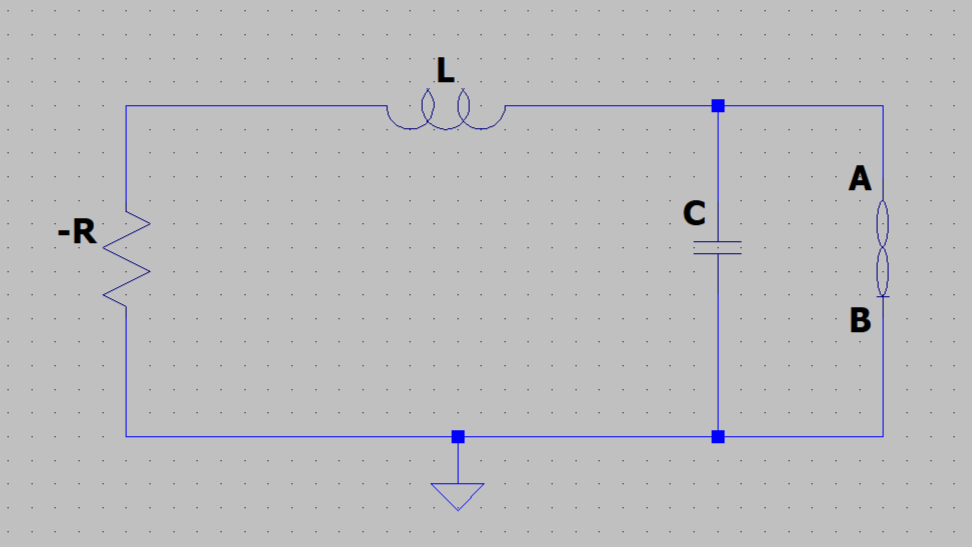
\includegraphics[width=0.7\textwidth]{-RLCM.png}
		\caption{Oscilador RLC con R negativa y Memristor.}
		\label{fig:-RLCM}
	\end{figure}
	
	Como se puede ver no existe una fuente de señal en el circuito y esto se debe a que el análisis hecho busca encontrar una oscilación periódica tan solo proporcionando condiciones iniciales a la bobina y el condensador, esto gracias al comportamiento de la resistencia negativa y del memristor los cuales se especifican mas adelante.
	
	\vspace{0.5cm}La forma de imponer las condiciones iniciales serían las clásicas, usando fuentes de intensidad en serie y tensión en paralelo con interruptores que se abren en \\$t\,=\,0(s)$ para la bobina y el condensador respectivamente.
	
	\newpage
	\section{Resistencia negativa}
	\noindent Uno de los componentes del circuito es la resistencia negativa la cual se puede construir con lo que se llama un \emph{Convertidor de Impedancia Negativa (NIC)}. Un NIC es un circuito activo, es decir, en lugar de disipar energía como una resistencia convencional, puede proporcionar energía a un circuito, ver \fref{fig:NIC}. En términos prácticos, un NIC puede ser utilizado para compensar la resistencia de carga de un sistema, mejorar la eficiencia de la transferencia de energía o realizar otras funciones específicas en circuitos eléctricos o electrónicos. En los circuitos osciladores, el NIC desempeña un papel importante en el mantenimiento, estabilización, frecuencia y calidad de la oscilación.
	 
	\begin{figure}[h]
		\centering
		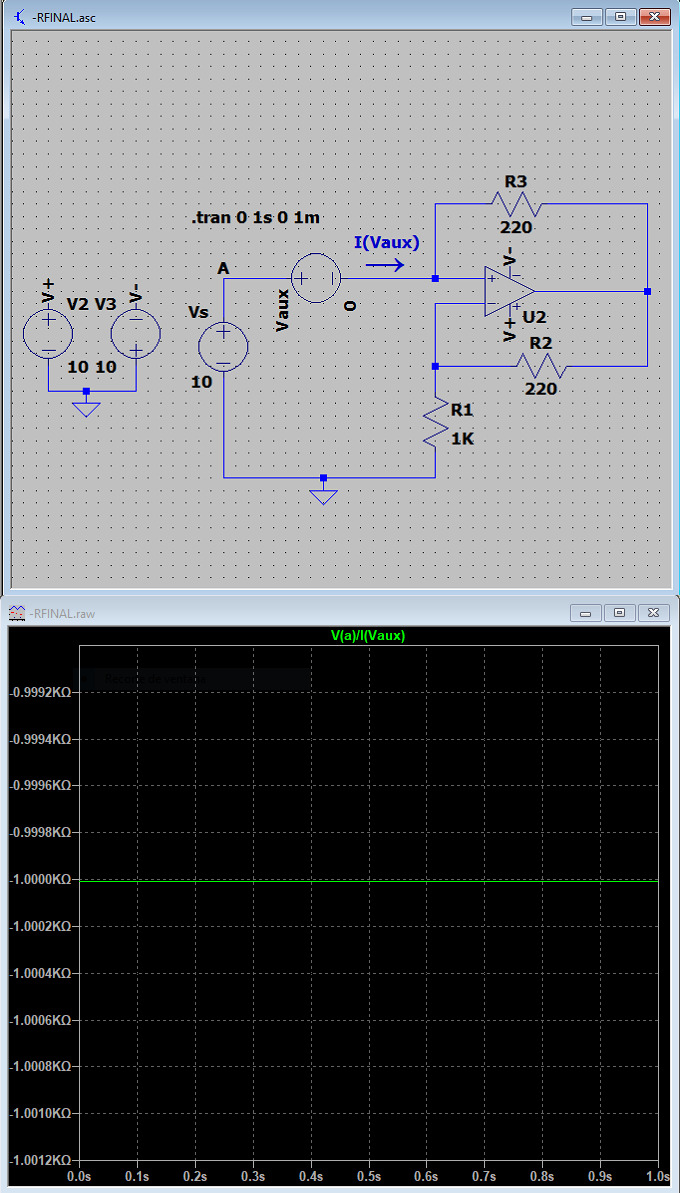
\includegraphics[width=0.65\textwidth]{NIC_B.jpg}
		\caption{Convertidor de Impedancia Negativa de -1000 Ohmios.}
		\label{fig:NIC}
	\end{figure}
	
	\newpage
	
	\noindent Una de las maneras de realizarlo es usando un amplificador operacional y 3 resistencias en la configuración que se ve en la \fref{fig:NIC} de esta manera si elegimos las resistencias $R_2=R_3$ la resistencia $R_1$ es la que determinaría el valor de resistencia negativa, esta es la explicación:
	
	\begin{center}
	\begin{multicols}{2}
		\centering
		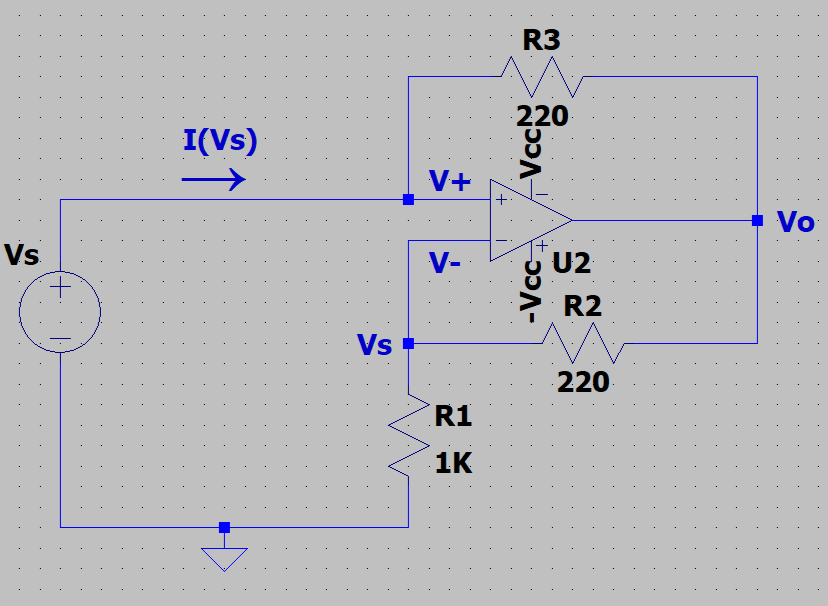
\includegraphics[width=\columnwidth]{demotracion_NIC.png}
		\captionof{figure}{Parámetros circuito NIC.}
		\label{fig:Param_NIC}
	
		\columnbreak
		
		Consideraciones para el cálculo del circuito de la \fref{fig:Param_NIC} con Amplificadores Operacionales:\\
		\begin{equation}
			V_+\,=\,V_-.
			\label{eq:NIC1}
		\end{equation}
		\begin{equation}
			I_+\,=\,I_-\,=\,0\,(A).
			\label{eq:NIC2}
		\end{equation}
	\end{multicols}
	\end{center}
	
	Si observamos la ecuación \eref{eq:NIC1} se puede ver que la tensión $V_S$ cae sobre la resistencia $R_1$ y se puede relacionar con la tensión de salida $V_O$ mediante un divisor de tensión:
	
	\begin{equation}
		V_S\,=\,V_O\,\frac{R_1}{R_1 + R_2}\:\longrightarrow\:V_O\,=\,V_S\,\frac{R_1 + R_2}{R_1}.
		\label{eq:NIC3}
	\end{equation}\smallskip
	
	Teniendo en cuenta la ecuación \eref{eq:NIC2} se puede ver que la intensidad $I(V_S)$ es la misma que pasa por la resistencia $R_3$, por ello se puede deducir:
	
	\begin{equation}
		I(V_S)\,=\,\frac{V_S - V_O}{R_3}.
		\label{eq:NIC4}
	\end{equation}\smallskip
	
	Sustituyendo la ecuación \eref{eq:NIC3} en \eref{eq:NIC4} y trabajando la expresión para obtener la relacion tensión-intensidad llegamos a:
	
	\begin{equation}
		I(V_S)\,=V_S\,\frac{-R_2}{R_1 \, R_3}.
		\label{eq:NIC5}
	\end{equation}\smallskip
	
	Si dividimos la tensión $V_S$ entre la intensidad $I(V_S)$ (ecuación \eref{eq:NIC5}) para obtener la impedancia de entrada del circuito:
	
	\begin{equation}
		\frac{V_S}{I(V_S)}\,=\,Z_{IN}\,=\,\frac{V_S}{V_S\,\frac{-R_2}{R_1 \, R_3}}\,=\,-R_1\,\frac{R_3}{R_2}.
		\label{eq:NIC6}
	\end{equation}\smallskip
	
	Si elegimos las resistencias $R_3\,=\,R_2$ en la ecuación \eref{eq:NIC6} obtenemos:
	
	\begin{equation}
		Z_{IN}\,=\,-R_1.
		\label{eq:NIC7}
	\end{equation}\smallskip
	
	\newpage
	\section{Memristor}
	\noindent El componente más interesante de este circuito es el Memristor, teorizado por el científico Leon Chua en 1971, ver \cite{chuamissing1971}. Este elemento trata de llenar el vacío que existía en las relaciones entre las cuatro variables básicas en teoría de circuitos: voltaje \textbf{\textit{v}}, intensidad \textbf{\textit{i}}, carga eléctrica \textbf{\textit{q}} y flujo magnético \textit{$\bm{\varphi}$}. En concreto el memristor relaciona la carga eléctrica con el flujo magnético de la siguiente manera, ver \cite{chuaoscillator2008}:
	
	\begin{equation}
		\varphi\,=\,\varphi(q), \qquad q\,=\,q(\varphi).
		\label{eq:flujocarga}
	\end{equation}\smallskip
	
	Sabiendo la relación del voltaje y la intensidad respecto a la carga y al flujo en el tiempo:

	\begin{equation}
		v(t)\,=\,\frac{d\varphi}{dt}, \qquad i(t)\,=\,\frac{dq}{dt}.
		\label{eq:dvdi}
	\end{equation}
			
	\begin{equation}
		\varphi(t)\,=\,\int_{-\infty}^{t}v(\tau)d\tau, \qquad q(t)\,=\,\int_{-\infty}^{t}i(\tau)d\tau.
		\label{eq:flujocargaintegral}
	\end{equation}\smallskip
	
	Derivando la ecuación \eref{eq:flujocarga} respecto al tiempo, y aplicando la regla de la cadena:
	
	\begin{equation}
		\frac{d\varphi}{dt}\,=\,\frac{d\varphi(q)\,dq}{dq\,dt}, \qquad \frac{dq}{dt}\,=\,\frac{dq(\varphi)\,d\varphi}{d\varphi\,dt}.
		\label{eq:vym}
	\end{equation}\smallskip
	
	Sustituyendo las relación de la ecuación \eref{eq:dvdi} en la ecuación \eref{eq:vym}:
	
	\begin{equation}
		v(t)\,=\,\frac{d\varphi(q)}{dq}i(t), \qquad i(t)\,=\,\frac{dq(\varphi)}{d\varphi}v(t).
		\label{eq:vym2}
	\end{equation}\smallskip
	
	Las dos relaciones de carga y flujo que quedan en la ecuación \eref{eq:vym2} son los que se denominan \textbf{\textit{Memristancia M(q)}} y \textbf{\textit{Memductancia W($\bm{\varphi}$)}}: 
	
	\begin{equation}
		M(q)\,=\,\frac{d\varphi(q)}{dq}, \qquad W(\varphi)\,=\,\frac{dq(\varphi)}{d\varphi}.
		\label{eq:myw}
	\end{equation}\smallskip
	
	Finalmente se presentan dos tipos de expresiones:
	
	\begin{equation}
		\textit{Memristor controlado por carga} \, \rightarrow \, v(t)\,=\,M(q)\,i(t).
		\label{eq:cc}
	\end{equation}\smallskip
	\begin{equation}
		\textit{Memristor controlado por flujo} \, \rightarrow \, i(t)\,=\,W(\varphi)\,v(t).
		\label{eq:fc}
	\end{equation}\smallskip

	
	
	\newpage
	
	\noindent El segundo acontecimiento más importante en relación al memristor fue en 2008 cuando en los laboratorios de HP se fabricó un componente cuyo comportamiento era muy parecido al funcionamiento que afirmaba Chua, debía de tener el memristor. En un inicio al componente que HP creó en 2005 le dieron el nombre de \textit{Crossbar Latch}, no sería hasta 2008 que se percataron de la similitud de funcionaminto con el memristor de Chua. La construcción es secilla, se trata de dos capas, una de dioxido de titanio puro y otra de dioxido de titanio deficiente de átomos de oxígeno, ambas envueltas por dos electrodos de platino \fref{fig:mem1}.\textit{\textcolor{red}{Repasar este párrafo, la frase de "debía tener..." quitar}}
	
	\begin{figure}[h]
		\centering
		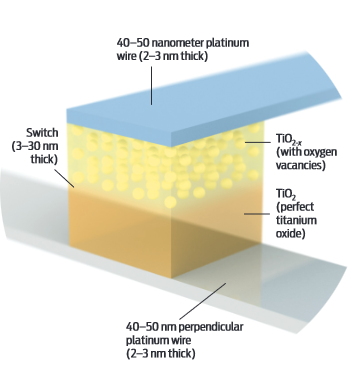
\includegraphics[width=0.6\textwidth]{mem1.png}
		\caption{Costruccion del memristor de HP. Ver \cite{williams}.}
		\label{fig:mem1}
	\end{figure}
	
	El óxido de titanio tiene una serie de características que lo hacen un material muy interesante en esta aplicación:
	\begin{enumerate}
		\item Resistencia variable: La resistencia eléctrica del óxido de titanio puede cambiar en repuesta de la aplicación de una corriente o un campo eléctrico. Lo cual nos permite no tan solo guardar 1 o 0 si no un rango de valores dentro de unos límites de operación.
		\item No volatilidad: El óxido de titanio puede mantener su estado de resistencia incluso cuando se retira la corriente eléctrica que lo atraviesa. Esto significa que puede retener información y mantener su estado de resistencia sin requerir energía continua.
		\item Cambios rápidos de resistencia:  Esta propiedad permite operaciones de escritura y lectura rápidas en el memristor, lo que es crucial para su uso en aplicaciones de almacenamiento y procesamiento de datos.
		\item Baja potencia y tamaño compacto
	\end{enumerate}
	\newpage
	
	La fórmula que se propone en \cite{HP} para modelar el comportamiento de este dispositivo es:
	
	\begin{equation}
		v(t)\,=\,\left(R_{ON}\,\frac{w(t)}{D}+R_{OFF}\left(1-\frac{w(t)}{D}\right)\right)i(t),
		\label{eq:hp1}
	\end{equation}
	
	\begin{equation}
		\frac{dw(t)}{dt}\,=\,\mu_V\,\frac{R_{ON}}{D}\,q(t).
		\label{eq:hp2}
	\end{equation}\smallskip
	
	Integrando la ecuación \eref{eq:hp2} e insertándola en \eref{eq:hp1} teniendo en cuenta que el valor de resistencia  $R_{ON} \ll R_{OFF}$: 
	
	\begin{equation}
		w(t)\,=\,\mu_V\,\frac{R_{ON}}{D}\,i(t),
		\label{eq:hp3}
	\end{equation}\smallskip
	\begin{equation}
		M(q)\,=\,R_{OFF}\,\left(1-\,\frac{\mu_V\,R_{ON}}{D^2}\,q(t)\right).
		\label{eq:hp4}
	\end{equation}\smallskip
	
	\begin{figure}[h]
		\centering
		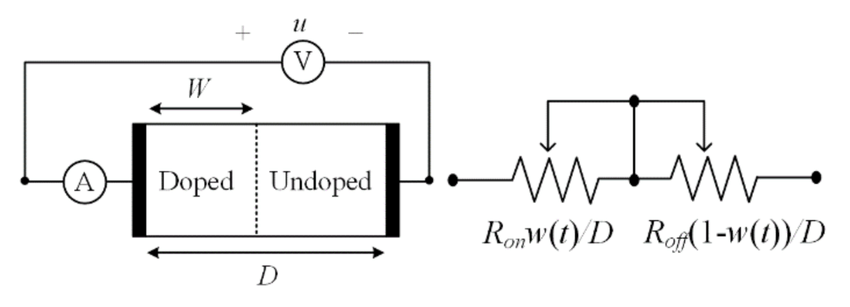
\includegraphics[width=1\textwidth]{schmem.png}
		\caption{Esquema del memristor de HP. Ver \cite{2021}.}
		\label{fig:2021}
	\end{figure}\smallskip
	
	Los parámetros que aparecen en las ecuaciones anteriores y que describen el funcionamiento del componente son:
	
	\begin{enumerate}
		\item $R_{ON}$: Resistencia en el estado ON, valor mínimo. Es constante.
		\item $R_{OFF}$: Resistencia en el estado OFF, valor máximo. Es constante.
		\item $\mu_V$: Mobilidad iónica de arrastre promedio. Es constante.
		\item $w$: Ancho de la zona dopada, no es constante, depende de la excitación.
		\item $D$: Ancho total de la lamina de oxido de titanio. Es constante.
	\end{enumerate}
	\newpage
	
	El funcionamiento es el siguiente, entre los dos electrodos de platino tenemos una capa de dióxido de titanio puro $TiO_2$ que actúa como dieléctrico y otra de dióxido de titanio con vacantes de oxígeno $TiO_{2-x}$ que actúa como conductor ya que en estas vacantes están cargadas positivamente (ver \fref{fig:mem1}), ya que al faltar átomos de oxígeno se están perdiendo también sus electrones de valencia asociados, generando así que el compuesto necesite atraer electrones a dichas vacantes para así mantenerse eléctricamente estable.Cuando un voltaje positivo se aplica al electrodo superior las vacantes de oxígeno de la zona dopada se repelen y viajan hacia la zona de óxido de titanio puro, haciendo así que aumente la conductividad hasta que se alcance el valor de $R_{ON}$. Si por el contrario el voltaje aplicado es negativo, las vacantes de oxígeno viajan hacia el elctrodo superior, reduciendo la conductividad hasta $R_{OFF}$.\textit{\textcolor{red}{Repasar este párrafo}}
	
	\begin{figure}[h]
		\centering
		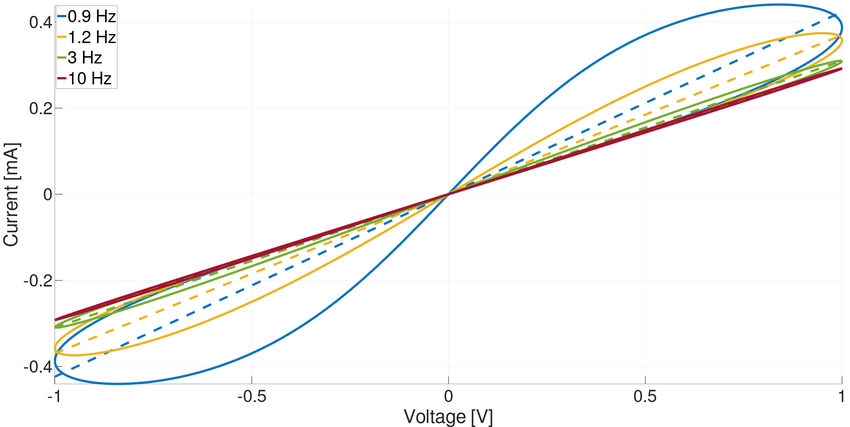
\includegraphics[width=0.8\textwidth]{iv_chua.png}
		\caption{Gráfica Tensión-Intensidad del Memristor de Chua ideal para una señal de entrada senoidal con varias frecuencias. Como se puede ver conforme aumenta la frecuencia la gráfica se parece más a la de una resistencia tradicional. Ver \cite{outsiders}}.
		\label{fig:iv_chua}
	\end{figure}\smallskip
	
		\begin{figure}[h]
		\centering
		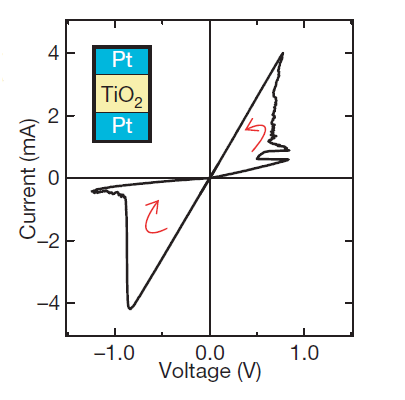
\includegraphics[width=0.5\textwidth]{iv_hp.png}
		\caption{Gráfica Tensión-Intensidad del Memristor de HP. Ver \cite{HP}.}
		\label{fig:iv_hp}
	\end{figure}\smallskip
	
	\newpage
	
	\section{Variables de estado}
	\noindent En este trabajo hemos hecho un análisis matemático de la bifurcación del circuito oscilador haciendo uso de técnicas de análisis de reciente estudio, pero primero hay que presentar el circuito y transformar sus ecuaciones eléctricas hasta llegar a una forma matemática con la que poder trabajar. Empecemos analizando el circuito.
	
	\begin{figure}[h]
		\centering
		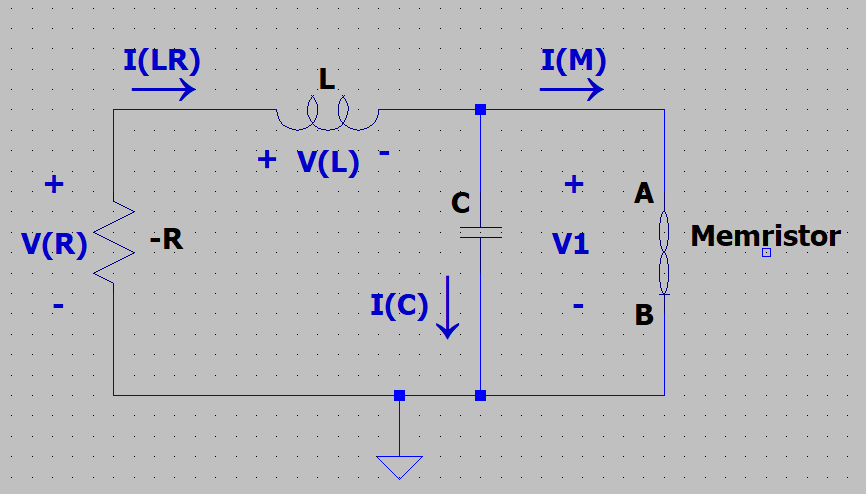
\includegraphics[width=0.8\textwidth]{circuito.png}
		\caption{Magnitudes del circuito.}
		\label{fig:circuito}
	\end{figure}\smallskip
	
	Aplicanco las leyes de Kirchoff a nuestro circuito, \fref{fig:circuito}, se puede ver que:
	
	\begin{equation}
		i_{LR}\,=\,i_M+i_C,
		\label{eq:kir1}
	\end{equation}
	\begin{equation}
		v_R\,=\,v_L+v_1.
		\label{eq:kir2}
	\end{equation}
	
	Reordenando las anteriores ecuaciones:
	
	\begin{equation}
		i_C\,=\,i_{LR}-i_M,
		\label{eq:kir11}
	\end{equation}
	\begin{equation}
		v_L\,=\,v_R-v_1.
		\label{eq:kir22}
	\end{equation}
	
	Recordando la relación entre la carga y el flujo con la intensidad y la tensión de las ecuaciones \eref{eq:dvdi}, la ecuación del memristor controlado por flujo \eref{eq:fc} y aplicándolo a \eref{eq:kir11} y \eref{eq:kir22} obtenemos:
	
	
	\begin{eqnarray}
		C\,\frac{dv_1}{dt}\,&=&\,i_{LR}-W(\varphi)\,v_1 \label{eq:kir111}, \\ [2mm]
		L\,\frac{di_{LR}}{dt}\,&=&\,R\,i_{LR}-v_1 \label{eq:kir222}, \\ [2mm]
		\frac{d\varphi}{dt}\,&=&\,v_1. \label{eq:kir333}
	\end{eqnarray}\smallskip
	
	Como se pueden ver las variables de estado elegidas son la intensidad en la resistencia y la bobina \bm{$i_{LR}$}, la tensión en el condensador y el memristor \bm{$v_1$} y el flujo en el memristor \bm{$\varphi$}.
	\newpage
	Reordenando las ecuaciones anteriores \eref{eq:kir111}, \eref{eq:kir222} y \eref{eq:kir333} tenemos:
	
	\begin{eqnarray}
		\frac{dv_1}{dt}\,&=&\,\frac{i_{LR}}{C}-W(\varphi)\,\frac{v_1}{C} \label{eq:sis1}, \\ [2mm]
		\frac{di_{LR}}{dt}\,&=&\,\frac{R}{L}\,i_{LR}-\frac{v_1}{L} \label{eq:sis2}, \\ [2mm]
		\frac{d\varphi}{dt}\,&=&\,v_1. \label{eq:sis3}
	\end{eqnarray}\smallskip
	
	Haciendo algunos cambios a las tres anteriores ecuaciones para luego poder trabajar con las ecuaciones obtenemos el siguiente sistema:
    
	\begin{equation}
		\label{eq:sistema1}
		\scalebox{1.2}{$\displaystyle
			\left\{
			\begin{aligned}
				\frac{dx}{dt} &= \alpha (y - W(z)x), \\
				\frac{dy}{dt} &= -\xi x + \beta y, \\
				\frac{dz}{dt} &= x.
			\end{aligned}
			\right.
			$}
	\end{equation}\smallskip
	
	Donde tenemos:
	\begin{equation*}
		x\,=\,v_1, \qquad y\,=\,i_{LR}, \qquad z\,=\,\varphi, \qquad \alpha\,=\,\frac{1}{C}, \qquad \beta\,=\,\frac{R}{L}, \qquad \xi\,=\,\frac{1}{L}.
	\end{equation*}
	
	Escribiendo el sistema \eref{eq:sistema1} de una forma más general:
	
	\begin{equation}
		\label{eq:sistema}
		\scalebox{1.2}{$\displaystyle
			\left\{
			\begin{aligned}
				\frac{dx}{dt} &= a_{11}W(z)x+a_{12}y, \\
				\frac{dy}{dt} &=  a_{21}x+ a_{22}y, \\
				\frac{dz}{dt} &= x.
			\end{aligned}
			\right.
			$}
	\end{equation}\smallskip
	
	Con:
	\begin{equation}
		\label{eq:amatriz}
	\begin{gathered}
		a_{11}=-\alpha=-\frac{1}{C}, \qquad a_{12}=\alpha=\frac{1}{C},\\[2mm]
		a_{21}=-\xi =-\frac{1}{L}, \qquad a_{22}=\beta = \frac{R}{L}.
	\end{gathered}
	\end{equation}\smallskip
	
	Pero del sistema \eref{eq:sistema} aun tenemos que definir $W(z)$. En \cite{chuaoscillator2008} se asume que el comportamiento del memristor se puede aproximar por una ecuacion linear a trozos monótonamente creciente:
	
	\begin{equation}
		q(\varphi)\,=\,b\varphi+0.5(a-b)(|\varphi+1|-|\varphi-1|).
		\label{eq:qf}
	\end{equation}
    \begin{center}
    	$ donde \quad a,b,c,d> 0$
    \end{center}
    
    Escribiendo \eref{eq:qf} con la variable \bm{$z$} y derivándola (recordando la ecuación \eref{eq:myw}) para obtener $W(z)$:
    
    \begin{equation}
    	q(z)\,=\,bz+0.5(a-b)(|z+1|-|z-1|),
    	\label{eq:qfz}
    \end{equation}
    
    \begin{equation}
    	W(z)\,=\,\frac{dq(z)}{dz}\,=\,
    		\label{eq:wz}
    		\scalebox{1}{$\displaystyle
    			\left\{
    			\begin{aligned}
    				a, \quad   |z| < 1,\\
    				b, \quad   |z| > 1.
    			\end{aligned}
    			\right.
    			$}
    \end{equation}\smallskip
    
    Por último vamos a definir dos matrices auxiliares del sistema \eref{eq:sistema} teniendo en cuenta la función $W(z)$ \eref{eq:wz}
    
    \begin{equation}
    	A_L=\begin{pmatrix*}[c]
    		a \, \cdotp a_{11} & a_{12}\\
    	             a_{21} & a_{22}\\
    	\end{pmatrix*}, \qquad 	A_R=\begin{pmatrix*}
    	b \, \cdotp a_{11} & a_{12}\\
    	a_{21} & a_{22}\\
    	\end{pmatrix*}.
    \end{equation}\smallskip
    
    con sus correspondientes trazas y determinantes:
    \begin{equation}
    \begin{aligned}
    	t_L &= a \cdot a_{11} + a_{22}\\
    	d_L &= a \cdot a_{11}a_{22} - a_{21}a_{12}\\
    	t_R &= b \cdot a_{11} + a_{22}\\
    	d_R &= b \cdot a_{11}a_{22} - a_{21}a_{12}\\
    \end{aligned}
    \end{equation}\smallskip
    
	Ya tenemos las ecuaciones necesarias para empezar el análisis, pero primero veremos en los siguientes capitulos que técnicas estaremos usando para ello.
	\newpage
	\section{Superficies invariantes}
	\noindent Lo que en teoría de bifurcaciones se denomina \textit{Superficie} o \textit{Plano} es un espacio topológico de dimensión $n$, en un sistema dinámico, cuyas propiedades de dicha superficie se mantienen inalteradas bajo la evolución de sistema. Es decir, es una región del espacio de fase donde las trayectorias de las soluciones del sistema permanecen contenidas, siempre que no aparezcan bifurcaciones de escape, pero no será nuestro caso. En este trabajo nos interesa estudiar los planos invariantes del sistema \eref{eq:sistema} ya que será donde aparecerá la órbita periódica que estamos buscando en nuestro circuito.
	
	\begin{definicion}
		Considerando el sistema diferencial:
		
		\begin{equation}
			\frac{dX}{dt}=F(X),\qquad X\in \mathbb{R}^3
		\end{equation}\smallskip
		Se dice que la superficie $S\subset \mathbb{R}^3$ es una superficie invariante, del sistema si la solución del sistema diferencial $X(t)$ con condición inicial $X(0)=X_0\; \in \; S$ satisface que $X(t) \in S$ para todo $t$.
	\end{definicion}
	
	\begin{figure}[h]
		\centering
		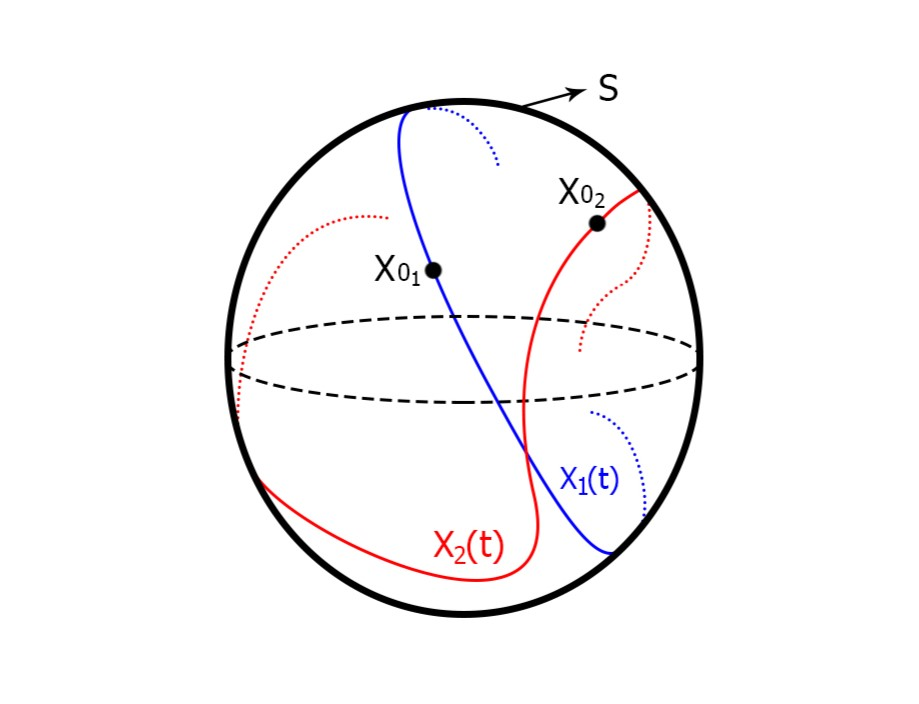
\includegraphics[width=1\textwidth]{esfera.jpg}
		\caption{Una esfera (que es una superficie $S\subset \mathbb{R}^3$) con una órbita solución, $X(t)$ con condición inicial $X(0)=X_0$, contenida en ella.}
		\label{fig:esfera}
	\end{figure}\smallskip
	\newpage
	
	Como se demuestra en el teorema 1 de \cite{ponce} existe un conjunto de superficies invariantes para nuestro sistema \eref{eq:sistema}, se enunciará dicho teorema en este trabajo ya que nos será muy importante tenerlo presente.
	
	\begin{theorem}
		\label{teorema1}
		Considerando el sistema \eref{eq:sistema} con la función lineal a trozos $q$ \eref{eq:qf} y la función $W(z)$ (posiblemente discontinua) \eref{eq:wz}. Para cualquier $h \in \mathbb{R}$, el conjunto:
		
		\begin{equation}
			\label{eq:sh}
			S_h=\left\{(x,y,z)\in \mathbb{R}^3\: : \: H(x,y,z)=h \right\}
		\end{equation}\smallskip
		
		\noindent es una superficiente invariante para el sistema, y se calcula con la siguiente expresión:
		\begin{equation}
			\label{eq:hecuation}
			H(x,y,z)=-a_{22}x+a_{12}y-a_{12}a_{21}z+a_{11}a_{22}q(z).
		\end{equation}\smallskip
		
		\noindent Además, el sistema tiene una familia infinita de superficies invariantes en todo $\mathbb{R}^3$, y la dinámica de los mismos es fundamentalmente bidimensional.
		
		\vspace{0.5cm}\noindent \textbf{Demostración:} Para cualquier solución $(\overline{x}(t),\overline{y}(t),\overline{z}(t))$ del sistema \eref{eq:sistema}, tenemos la función $h(t)=H(\overline{x}(t),\overline{y}(t),\overline{z}(t))$. Si derivamos $h(t)$ y sustituimos las ecuaciones de las tres incógnitas:\textit{\textcolor{red}{REPASAR AL ECUACIÓN, ESTA BIEN HECHA LA DERIVACIÓN? SE VA TODO Y QUEDA 0? MIRAR ARTICULO PONCE}}
		
		\begin{equation}
				h'=-a_{22}(a_{11}W(z)+a_{12}y)+a_{12}(a_{21}x+a_{22}y)+(a_{11}a_{22}W(z)-a_{12}a_{21})x=0.
		\end{equation}\smallskip

		\noindent por lo que $h$ es constante a lo largo de toda la órbita y por lo tanto invariante a la dinámica del sistema.
	\end{theorem}
	
	Como se ha dicho en el teorema anterior la dinamica de estas superficies se puede reducir a un comportamiento bidimensional, esto se demuestra en el teorema 2 de \cite{ponce}, nuevamente lo enunciaremos pues nos interesa tenerlO presente. Lo que se hace en este teorema es mediante el cambio de variable adecuado transformar nuestro sistema de tres variables en uno de dos variable.
	
	\newpage
	
	\begin{theorem}
		Considerando el sistema \eref{eq:sistema}, la función $W(z)$ \eref{eq:wz} con $a\neq b$ y tomando la hipótesis $a_{22}=\frac{R}{L}\neq 0$, la dinámica del sistema \eref{eq:sistema} es topologicamente equivalente a la dinamica del sistema lineal a trozos de dimensión 2
		
		\begin{equation}
			\label{eq:sis2ec}
			\begin{gathered}
				\dot{\tilde{x}}=F(\tilde{x})-\tilde{y}, \\[2mm]
				\dot{\tilde{y}}=g(\tilde{x})-h,
			\end{gathered}
		\end{equation}
		
		con
		
		\begin{equation}
			\label{f1}
			F(\tilde{x})=
			\left\{
			\begin{aligned}
				&t_R(\tilde{x}-1)+t_L, \quad &si& \quad \tilde{x}>1,\\
				&t_L\tilde{x}, &si& \quad |\tilde{x}|\leq 1,\\
				&t_R(\tilde{x}+1)-t_L, \quad &si& \quad \tilde{x}<-1,
			\end{aligned}
			\right.
		\end{equation}\smallskip
		
		\begin{equation}
			\label{eq:g1}
			F(\tilde{x})=
			\left\{
			\begin{aligned}
				&d_R(\tilde{x}-1)+d_L, \quad &si& \quad \tilde{x}>1,\\
				&d_L\tilde{x}, &si& \quad |\tilde{x}|\leq 1,\\
				&d_R(\tilde{x}+1)-d_L, \quad &si& \quad \tilde{x}<-1.
			\end{aligned}
			\right.
		\end{equation}\smallskip
		
		\vspace{0.5cm}\noindent \textbf{Demostración:} Cuando $a_{22}\neq0$ en el sistema \eref{eq:sistema} podemos solucionar la ecuación $H(x,y,z)=h$ \eref{eq:hecuation} para $x$, escribiendo:
		
		\begin{equation}
			\label{eq:xeqn}
			x=\frac{a_{12}}{a_{22}}y+a_{11}q(z)-\frac{a_{12}a_{21}}{a_{22}}z-\frac{h}{a_{22}}.
		\end{equation}\smallskip
		
		Ssutituyendo la ecuación \eref{eq:xeqn} en la segunda y tercera ecuación de \eref{eq:sistema}, tenemos:
		
		\begin{equation}
			\label{eq:cambyz}
			\begin{aligned}
				&\dot{y}=\alpha_1y-\alpha_2z+a_{11}a_{21}q(z)-\frac{a_{21}h}{a_{22}}, \\[2mm]
				&\dot{z}=\alpha_3y-\alpha_4z+a_{11}q(z)-\frac{h}{a_{22}}.
			\end{aligned}
		\end{equation}
		
		con
		
		\begin{equation}
			\label{eq:alphamatriz}
			\begin{aligned}
				&\alpha_1=\frac{a_{22}^2+a_{12}a_{21}}{a_{22}}, \qquad &\alpha_2=\frac{a_{21}^2a_{12}}{a_{22}},\\[2mm]
				&\alpha_3=\frac{a_{12}}{a_{22}}, \qquad &\alpha_4=\frac{a_{12}a_{21}}{a_{22}}.
			\end{aligned}
		\end{equation}\smallskip
		
		Seguidamente considerando el siguiente cambio de variable
		
		\begin{equation}
			\label{eq:xytilde}
			\begin{aligned}
				&\tilde{x}=z, \\[2mm]
				&\tilde{y}=\alpha_1z-\alpha_3y+\frac{h}{a_{22}}
			\end{aligned}
		\end{equation}\smallskip
		
		 el sistema \eref{eq:cambyz} se puede escribir en la forma \eref{eq:sis2ec}-\eref{eq:g1}.
		
	\end{theorem}
	
	\vspace{0.5cm}Una breve explicación de los anteriores teoremas. Siempre que $a_{22}\neq 0$, si elegimos una condición inicial de nuestro sistema que se encuentre dentro de alguna superficie de las que hemos definido en \eref{eq:sh}, y las cuales podemos calcular con la expresión \eref{eq:hecuation} con las condiciones iniciales de $x,y,z$, entonces la solución del sistema siempre estará contenida en dicha superficie. Es decir, mirando las ecuaciones \eref{eq:xytilde}; con $\tilde{x}$ calculamos la $z$, con $\tilde{y}$ podemos despejar y calcular la $y$ (recordemos que $h$ ya la hemos definido con las condiciones iniciales), y finalmente con la ecuación \eref{eq:xeqn} calculamos la $x$ .Hemos reducido un sistema tridimensional a uno bidimensional y conocemos el plano $h$ donde estará contenia la solución del sistema, solución que estamos buscando que sea una órbita periódica.
	
	\vspace{0.5cm}Como dijimos en el teorema \ref{teorema1}, la función $W(z)$ puede ser discontinua, esto dependerá de las carácterísticas del memristor. Aún así esta posible discontinuidad no nos afectará en nuestro trabajo como se demuestra en la sección 3 de \cite{ponce} donde los autores demuestran como pasar en cualquier caso de un modelo discontinuo a un modelo reducido continuo. Además en el artículo de Chua de 2008, ver \cite{chuaoscillator2008} donde se presenta el circuito que estamos estudiando en este trabajo, los autores presentan una aproximación de lo que podrían ser la gráfica flujo-carga del memristor caracterizada por la ecuación \eref{eq:qfz}-\eref{eq:wz} y la suponen continua.
	
	\vspace{0.5cm}Además, nuestro nuevo sistema de dimensioón dos tiene tres zonas como vemos en \eref{eq:sis2ec}-\eref{eq:g1}, sin embargo en este trabajo nos centraremos en dos de ellas, puesto que buscaremos oscilaciones periódicas bizonales. Se hace esta aclaración puesto que parte del trabajo que haremos mas adelante, como la forma canónica de Lienard, nos permitiría hacer el estudio de tres zonas, pero no es nuestro objetivo.
	
	

	
	\chapter{Sistemas Dinámicos Continuos}
	En este capítulo haremos un repaso de sistemas dinámicos continuos lineales a trozos puesto que como hemos visto en el sistema \eref{eq:sistema} hemos reducido nuestro circuito a un sistema de este tipo. Lo que necesitamos ahora es encontrar la o las soluciones de nuestro sistema y estudiar su estabiliad, la base que necesitamos para ello lo veremos en este capítulo.
	\newpage
	\section{Sistemas lineales planos}
	\label{sec:sislinplanos}
	En esta sección vamos a analizar los sistemas dinámicos continuos de 2 ecuaciones lineales de primer orden con coeficientes constantes, ya que posteriormente describiremos nuestro circuito de esta forma.
	Antes que nada hay que definir lo que es un sistema dinámico continuo:
	
	\begin{definicion}
		Un sistema dinámico es un conjunto de ecuaciones de cambio que describen la evolución temporal de algún fenómeno, que puede ser de cualquier naturaleza (eléctrico, económico, cinegético...), de manera que el estado presente del sistema viene determinado por los estados anteriores. El estado del sistema queda descrito por sus variables de estado. Cuando la evolución se estudia considerando el tiempo como una variable 
		continua, decimos que el sistema es continuo y para analizar este tipo de sistemas la regla determinista que lo gobierna es su sistema de ecuaciones diferenciales.
	\end{definicion}
	
	Un sistema de este tipo tiene la siguiente forma:
	
	\begin{equation}
		\label{eq:edo2}
		\scalebox{1.2}{$\displaystyle
			\left\{
			\begin{aligned}
				\dot{x}\,=\,\frac{dx}{dt}\,=\,a_{11}x(t)+a_{12}y(t)+b_1 \\
				\dot{y}\,=\,\frac{dy}{dt}\,=\,a_{21}x(t)+a_{22}y(t)+b_2
			\end{aligned}
			\right.
			$}
	\end{equation}\smallskip
	
	Escribiendo el sistema \eref{eq:edo2} en forma matricial:
	
	\begin{equation}
		\label{eq:matrxedo2}
		\scalebox{1.2}{$\displaystyle
		\begin{pmatrix}
			\dot{x}\\
			\dot{y}\\
		\end{pmatrix} =
		\begin{pmatrix}
			a_{11} & a_{12}\\
		    a_{21} & a_{22}\\
		\end{pmatrix} 
		\begin{pmatrix}
			x\\
			y\\
		\end{pmatrix} + 
		\begin{pmatrix}
			b_1\\
			b_2\\
		\end{pmatrix}
		$}
	\end{equation} \smallskip
	
	Ecribiendo el sistema \eref{eq:matrxedo2} de forma mas simplificada:
	
	\begin{equation}
		\label{eq:sisautonomo}
		\dot{X}\,=\,AX+B
	\end{equation}\smallskip
	
	Cuando $B=\vec{0}$ el sistema se dice homogéneo. Por el contrario cuando $B\neq\vec{0}$ el sistema se dice no homogéneo. Esto es importante saberlo pues los métodos para solucionar estos tipos de sistemas no son las mismos.
	
	Tambien hay que tener en cuenta las condiciones iniciales del sistema:
	
	\begin{equation}
		\label{eq:ci}
		\scalebox{1.2}{$\displaystyle
			\left\{
			\begin{aligned}
				x(0)=x_0 \\
			    y(0)=y_0
			\end{aligned}
			\right.
			$}
	\end{equation}\smallskip
	
	Escribiendo el sistema \eref{eq:ci} en forma matricial:
	
	\begin{equation}
		\label{cimat}
		X(t_0)=\begin{pmatrix}
			x(0)\\y(0)
		\end{pmatrix}=\begin{pmatrix}
		x_0\\y_0
		\end{pmatrix}=X_0
	\end{equation}\smallskip
	
	Al conjunto del sistema y a sus condiciones iniciales se les denomina \\ \textbf{\textit{Problema de Valor Inicial (PVI)}}: 
	
	\begin{equation}
	\label{eq:pvi}
	\scalebox{1.2}{$\displaystyle
		\left\{
		\begin{aligned}
			&\dot{X}=AX+B &\rightarrow& \textit{Sistema Diferencial (S.D.)}\\
			&X(t_0)=X_0 &\rightarrow& \textit{Condiciones Iniciales (C.I.)}
		\end{aligned}
		\right.
		$}
    \end{equation}\smallskip
	
	Lo primero y más importante que se debe hacer con este tipo de problemas es comprobar la existencia y unicidad de sus soluciones.
	\newpage
	\begin{theorem}\label{thm:interesante}
		Existencia y unicidad \\[2mm]
		\textit{Sean $A$ y $B$ continuas en un intervalo $I\subseteq  \mathbb{R}$, que continene el punto $X(t_0)$ entonces el P.V.I. tiene una única solución definida en dicho intervalo $I$ para cualquier vector $X_0 \in \mathbb{R}^2$}. Además, si el P.V.I. tiene coeficientes constantes en $A$ y $B$ la solución está definida en $\mathbb{R}$.
	\end{theorem}
	\vspace{4mm}
	
	Las soluciones del sistema son el conjunto de puntos \eref{eq:puntos} para cada instante de tiempo que forman una curva en el plano de fases $xy$.
	\begin{equation}
		\label{eq:puntos}
		X(t)=\begin{pmatrix}
			x(t) \\ y(t)
		\end{pmatrix}
	\end{equation}\smallskip
	
	Ahora lo lógico sería hablar de como resolver este tipo de problemas ya que es nuetsro objetivo, pero no lo vamos a hacer ya que nosotros no usaremos el método tradicional de autovalores y autovectores para ello, vamos a utilizar otra técnica de reciente estudio con la que no hará falta esto, la veremos mas adelante.\\[0.5cm]
	Por último veamos como obtener y analizar los puntos de equilibrio del Sistema Lienal Plano. Primero escribamos el sistema \eref{eq:edo2} de otra forma para ver los siguientes apartados mejor:
	\begin{equation}
		\label{eq:sv}
		\scalebox{1.2}{$\displaystyle
			\left\{
			\begin{aligned}
				\dot{x}\,=\,\frac{dx}{dt}\,=S(x,y) \\
				\dot{y}\,=\,\frac{dy}{dt}\,=V(x,y)
			\end{aligned}
			\right.
			$}
	\end{equation}\smallskip
	
	\begin{definicion}
		Los puntos $(\overline{x},\overline{y})$ que anulan simultaneamente las funciones $S$ y $V$ del sistema \eref{eq:matrxedo2} se denominan Puntos de Equilibrio o Críticos del sistema:
	\end{definicion}

	\begin{eqnarray}
		\label{eq:crit}
			\begin{pmatrix}
				0\\
				0\\
			\end{pmatrix} =
			&\begin{pmatrix}
				a_{11} & a_{12}\\
				a_{21} & a_{22}\\
			\end{pmatrix}&
			\begin{pmatrix}
				\overline{x}\\
				\overline{y}\\
			\end{pmatrix} + 
			\begin{pmatrix}
				b_1\\
				b_2\\
			\end{pmatrix}\nonumber \\[4mm]
			&\begin{pmatrix}
			a_{11} & a_{12}\\
			a_{21} & a_{22}\\
			\end{pmatrix}&
			\begin{pmatrix}
			\overline{x}\\
			\overline{y}\\
			\end{pmatrix} = 
			\begin{pmatrix}
			-b_1\\
			-b_2\\
			\end{pmatrix} \nonumber \\[4mm]
			&A\,\overline{X}=-b
	\end{eqnarray}\smallskip
	
	Si el $det(A)\neq0$ \eref{eq:crit} el sistema posee un único punto de equilibrio, este punto se dice solucion constante del sistema.
    \\[0.5cm]
    Veamos esto más en profundiad, primero tenemos que saber que el sistema que tenemos \eref{eq:sv} se denomina \textit{\textbf{Autónomo}} ya que la variable independiente $\bm{t}$ no aparece de manera explícita en los segundos términos.
    \newpage
    Ahora lo que haremos es una translación del punto de equilibrio para que esté en el origen $\begin{pmatrix} 0 \\ 0
    \end{pmatrix}$ en caso de no estarlo:
    
	\begin{equation}
		\label{eq:trans}
		\scalebox{1.2}{$\displaystyle
			\left\{
			\begin{aligned}
				\tilde{X}=x-\overline{x} \\
				\tilde{Y}=y-\overline{y}
			\end{aligned}
			\right.
			$}
	\end{equation}\smallskip
	
	Por lo que ahora tenemos:
	
	\begin{equation}
		\label{eq:trans2}
		\scalebox{1.2}{$\displaystyle
			\left\{
			\begin{aligned}
				\frac{d\tilde{X}}{dt}\,=S(\tilde{X}-\overline{x},\tilde{Y}-\overline{x}) \\
				\frac{d\tilde{Y}}{dt}\,=V(\tilde{X}-\overline{x},\tilde{Y}-\overline{x})
			\end{aligned}
			\right.
			$}
	\end{equation}\smallskip
	Donde el punto $\begin{pmatrix} 0 \\ 0 \end{pmatrix}$ es el punto de equilibrio. \\[0.5cm]
	Lo que verermos a continuacion es la disposicion de las soluciones al rededor del punto de equilibrio y la estabilidiad o no del mismo. Considerando el sistema autónomo lineal con punto de equilibrio en el origen que hemos obtenido tras el cambio de variable:
	
	\begin{eqnarray}
		\label{eq:trans3}
			\begin{pmatrix}
				\dot{x}\\
				\dot{y}\\
			\end{pmatrix} =
			&\underbrace{\begin{pmatrix}
				a_{11} & a_{12}\\
				a_{21} & a_{22}\\
			\end{pmatrix}}&
			\begin{pmatrix}
				x\\
				y\\
			\end{pmatrix} \nonumber \\[1mm]
			&A&
	\end{eqnarray} \smallskip
	
	Como vemos con el cambio de variable no se ha modificado la matriz $A$ que es la que nos dirá todo respecto a la estabilidad del punto crítico, veremos los tres casos que se estudian en este trabajo: Foco Asintóticamente Estable, Foco Asintóticamente Inestable y Centro. Pero hay muchos mas y, por supuesto, combinaciones de todos ellos, lo cual complica estos problemas en gran medida.\\[0.5cm]
	Para saber la estabilidad de los puntos debemos estudiar el polinomio caracteristico de la matriz $A$:
	
	\begin{equation}
		\label{eq:equilibrio}
		A=\begin{pmatrix}
			a_{11} & a_{12}\\
			a_{21} & a_{22}\\
		\end{pmatrix}\rightarrow\left\{
		\begin{aligned}
		det(A )&= a_{11}a_{22}-a_{12}a_{21} \\
		tr(A) &= a_{11}+a_{22}
	    \end{aligned}
		\right.
	\end{equation}\smallskip
	
	\begin{eqnarray}
		\begin{aligned}
		P_A(\lambda)=&\lambda^2-tr(A)\lambda+det(A) \nonumber \\[1mm]
		&\lambda^2-tr(A)\lambda+det(A)=0 \nonumber \\[1mm]
		\textit{Autovalores}\rightarrow \quad &\lambda=\frac{tr(A)\pm \sqrt{tr(A)^2-4\,det(A)}}{2}
	    \end{aligned}
	\end{eqnarray}
	
	\newpage

	{\Large\textbullet\quad Foco Asintóticamente Estable}\\[0.5cm]
	
	Las curvas solucion tienden al punto crítico. Este caso se da para: 
	\begin{itemize}
		\item $\bm{tr(A)<0}$
		\item $\bm{tr(A)^2-4\,det(A)<0}$
	\end{itemize}
	
	\begin{figure}[h]
		\centering
		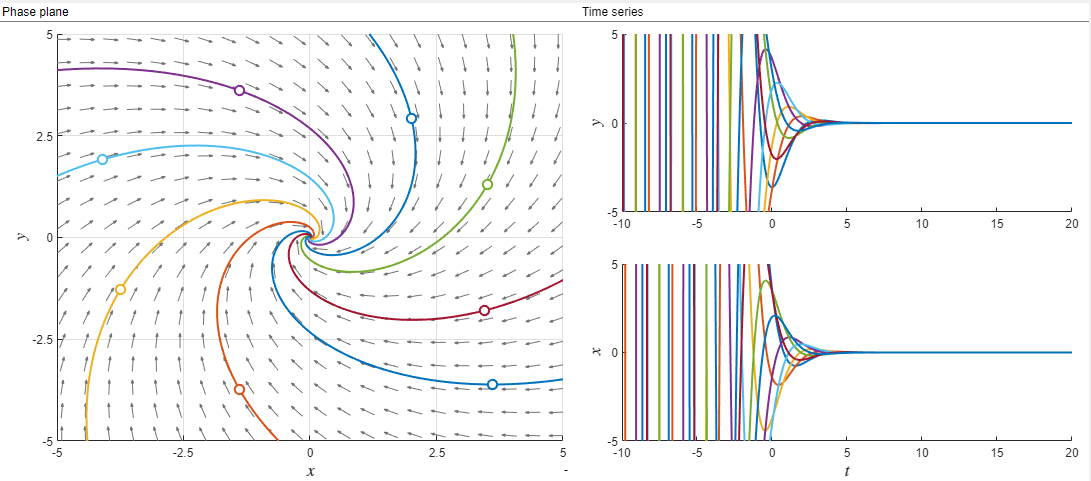
\includegraphics[width=1\textwidth]{estable.png}
		\caption{Foco Asintóticamente Estable visto en el plano de fases $xy$ (izquierda) y la variacion de $x$ e $y$ en el tiempo (derecha).}
		\label{fig:estable}
	\end{figure}\smallskip
	
	La matriz $A$ del la \fref{fig:estable} es 
	$\begin{pmatrix*}[r]
		-1 & 1 \\
		-1 & -1
	\end{pmatrix*}$
	
	\begin{align*}
		&\bullet\quad tr(A)=-2<0 \\[2mm]
		&\bullet\quad tr(A)^2-4\,det(A)=4-4(2)<0
	\end{align*}
	
	\newpage
	
	{\Large\textbullet\quad Foco Asintóticamente Inestable}\\[0.5cm]
	
	Las curvas solucion tienden al alejarse del punto crítico. Este caso se da para: 
	\begin{itemize}
		\item $\bm{tr(A)>0}$
		\item $\bm{tr(A)^2-4\,det(A)<0}$
	\end{itemize}
	
	\begin{figure}[h]
		\centering
		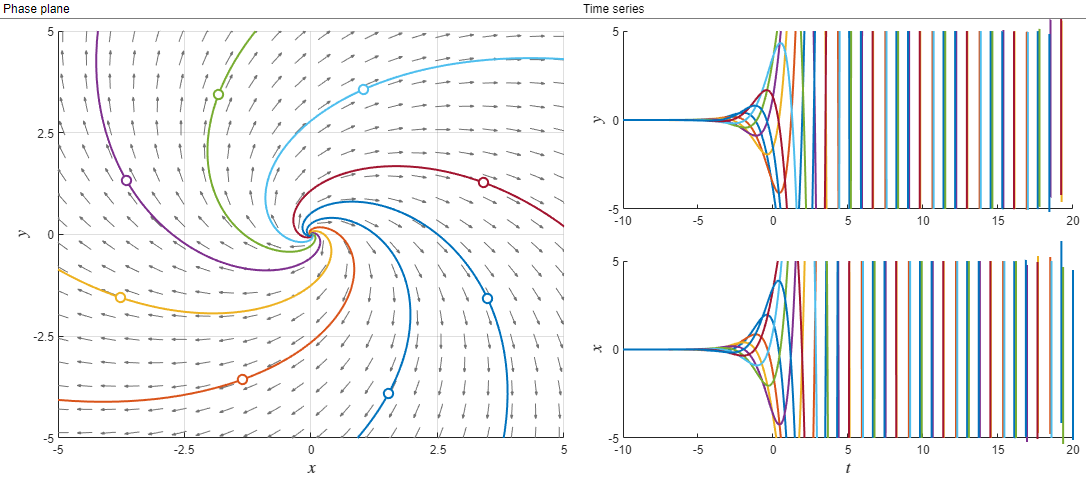
\includegraphics[width=1\textwidth]{inestable.png}
		\caption{Foco Asintóticamente Inestable visto en el plano de fases $xy$ (izquierda) y la variacion de $x$ e $y$ en el tiempo (derecha).}
		\label{fig:inestable}
	\end{figure}\smallskip
	
	La matriz $A$ del la \fref{fig:inestable} es 
	 $\begin{pmatrix*}[r]
		 1 & 1 \\
		-1 & 1
	 \end{pmatrix*}$
	
	\begin{align*}
		&\bullet\quad tr(A)=2>0 \\[2mm]
		&\bullet\quad tr(A)^2-4\,det(A)=4-4(2)<0
	\end{align*}
	
	\newpage
	
    {\Large\textbullet\quad Centro}\\[0.5cm]
    
    Las curvas solucion son concéntricas al punto crítico. Este caso se da para: 
    \begin{itemize}
    	\item $\bm{tr(A)=0}$
    	\item $\bm{tr(A)^2-4\,det(A)<0}$
    \end{itemize}
    
    \begin{figure}[h]
    	\centering
    	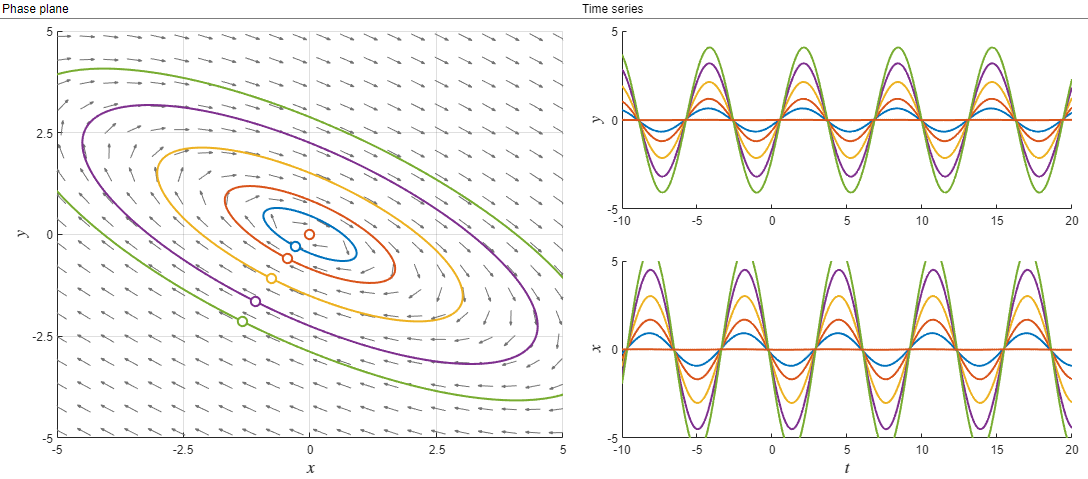
\includegraphics[width=1\textwidth]{centro.png}
    	\caption{Centro en el plano de fases $xy$ (izquierda) y la variacion de $x$ e $y$ en el tiempo (derecha).}
    	\label{fig:centro}
    \end{figure}\smallskip
    
    La matriz $A$ del la \fref{fig:centro} es 
    $\begin{pmatrix*}[r]
    	1 & 2 \\
    	-1 & -1
    \end{pmatrix*}$
    
    \begin{align*}
    	&\bullet\quad tr(A)=1-1=0 \\[2mm]
    	&\bullet\quad tr(A)^2-4\,det(A)=0-4(1)<0
    \end{align*}
	
	\newpage
	\section{Sistemas lineales a trozos bizonales}
	\label{sistrobiz}
	En esta sección vamos a ver como estudiar los sistemas continuos dinámicos lineales a trozos de dos zonas y veremos sus propiedades de cara a la obtención de una órbita periódica y estudiar su amplitud y periodo.\\[0.5cm] También veremos como utilizar las formas canónicas para reducir el número de parámetros que influyen en el sistema y como apoyarnos en dichas formas canónicas y las propiedades que nos portan a la hora de estudiar la oscilacion periódica de nuestro circuito.
	
	\begin{definicion}
		Un sistema dinámico continuo lineal a trozos plano con dos zonas es un sistema de ecuaciones diferenciales con la siguiente forma:
	\end{definicion}
	
	\begin{equation}
		\frac{dx}{dt}=\dot{x}=S(x)=
		\label{eq:biz1}
		\scalebox{1}{$\displaystyle
			\left\{
			\begin{aligned}
			 A_1x+b_1\quad si \quad x^T\cdotp w+\delta \leq 0 \\
			 A_2x+b_2\quad si \quad x^T\cdotp w+\delta < 0
			\end{aligned}
			\right.
			$}
	\end{equation}\smallskip
	Donde $x=(x_1,x_2)^T\in \mathbb{R}^2$, las matrices $A_1$ y $A_2$ son reales de orden $2$, además\\ $b_1$, $b_2$, $w$ $\in \mathbb{R}^2$ con $w\neq\vec{0}$ y $\delta \in \mathbb{R}$ y se satisface la condición de continuidad
	
	\begin{equation}
		A_1x+b_1=A_2x+b_2 
	\end{equation}\smallskip
	
	Sobre la recta de separación de las dos zonas:\quad $x^T\cdotp w+\delta = 0$ \\[0.5cm]
	
	\textbf{\textcolor{red}{EXISTENCIA Y UNICICDAD DE SISTEMA 3.14}}

	Para cada $x^0 \in \mathbb{R}^2$, el problema de valores iniciales \eref{eq:pvi2} tiene una solución única $x(t)$ definida para todo $t$ real.
	
	\begin{equation}
		\label{eq:pvi2}
		\scalebox{1.2}{$\displaystyle
			\left\{
			\begin{aligned}
				&\dot{x}=S(x)\\
				&x(0)=x^0
			\end{aligned}
			\right.
			$}
	\end{equation}\smallskip
	
	 A continuación veremos la forma canónica mas común para los sistemas bizonales que coloca la recta separación en el eje de ordenadas $x_1=0$.
	
	\begin{definicion}
		Todo sistema dinámico continuo lineal a trozos plano con dos zonas puede escribirse de la siguiente forma:
	
	\begin{equation}
		\dot{x}=S(x)=
		\label{eq:lien}
		\scalebox{1}{$\displaystyle
			\left\{
			\begin{aligned}
				B_1x+c\quad si \quad x_1 \leq 0 \\
				B_2x+c\quad si \quad x_1 < 0
			\end{aligned}
			\right.
			$}
	\end{equation}\smallskip
	\textbf{\textcolor{red}{$S(x)$? pero yo tengo dos variables x1 y x2, es $S(x_1,x_2)$? }}
	
	Con $x=(x_1,x_2)^T, c\in \mathbb{R}^2$ y las matrices $B_1$, $B_2$ comparten sus dos últimas columnas por continuidad, esto es:
	\begin{equation}
		B_1-B_2 = \left(B_1-B_2\right)e_1e_1^T 
	\end{equation}\smallskip
	
	\textbf{\textcolor{red}{multiplicado los e?}}
	
	Siendo $e_1=(1,0)^T$ el primer vector de la base canónica $\mathbb{R}^2$. Además, por continuidad también, se puede ver que $c_1=c_2=c$.
    \end{definicion}\smallskip

	
	\textbf{Demostración}: Basta con realizar una simetría para que el vector $w$ normal a la recta $x^T\cdotp w+\delta=0$, se transforme en el vector $e_1=(1,0)^T$ se puede hacer usando matrices de Householder \cite{docvic}. Por último con una translación hacemos que la nueva recta de separación $x_1=0$ (ahora vertical) pase por el origen. Por lo que el sistema queda con la forma:
	\textbf{\textcolor{red}{y que pasa con $\delta$? por que la recta se llama $x_1$, la puedo llamar solo x? menos lio con $\dot{x}_1$. Pero $x^T$ y $w$ son vectores? en lugar de la recta x=0 se podria usar la x=-1?}}
	
	\begin{equation}
		\dot{x}=
		\label{eq:lien2}
		\scalebox{1}{$\displaystyle
			\left\{
			\begin{aligned}
			B_1x+c_1\quad si \quad x_1 \leq 0 \\
			B_2x+c_2\quad si \quad x_1 < 0
			\end{aligned}
			\right.
			$}
	\end{equation}\smallskip
	
	Con $B_1$ y $B_2$ matrices de orden 2 y $c_1, c_2 \in \mathbb{R}^2$. Nuevamente por continuidad se debe satisfacer:
	
	\begin{equation}
		\label{eq:b1b2}
		B_1x+c_1=B_2x+c_2 \qquad si \quad x_1=0
	\end{equation}\smallskip
	
	Como el punto $(0,0)^T$ está en la recta de separación $x_1=0$, sustituyendo en \eref{eq:b1b2} se tiene que $c_1=c_2$ por lo que:
	
	\begin{equation}
		B_1x=B_2x \qquad si \quad x_1=0
	\end{equation}\smallskip
	
	Como el vector $(0,1)^T$ está sobre la recta de separación $x_1=0$, se tiene por tanto que las dos últimas columnas de $B_1$ y $B_2$ son iguales \textbf{\textcolor{red}{????}}, y además no olvidemos que  antes hemos visto que $c_1=c_2=c$.
	\\ [0.5cm]
	Se ha reducido bastante el número de parámetros, ahora tenemos 8, 6 de ellos vienen de las matrices $B_1$ y $B_2$ y 2 de $c$. Para seguir reduciendo parámetros tengamos en cuenta que estamos buscando oscilaciones y que no aparecerán en sistemas unidimensionales por lo que el primer término de las segundas columnas de las matrices $B_1$ y $B_2$ no puede ser nulo (condición de observabilidad \cite{onsimplyfing}). Mediante el cambio de variable oportuno lo convertiremos en $(-1)$ aquí lo vemos, en primer lugar escribimos el sistema \eref{eq:lien2} de la siguiente manera:
	
	\begin{equation}
		\begin{pmatrix*}[r]
			\dot{x}_1 \\ \dot{x}_2
		\end{pmatrix*}=
		\label{eq:lie-1}
		\scalebox{1.2}{$\displaystyle
			\left\{
			\begin{aligned}
				\begin{pmatrix*}[r]
					b_{11}^1 & b_{12} \\
					b_{21}^1 & b_{22}
				\end{pmatrix*}\begin{pmatrix*}[r]
				x_1\\x_2
				\end{pmatrix*}+\begin{pmatrix*}[r]
				c_1 \\ c_2
				\end{pmatrix*} \quad si \quad x_1 \leq 0 \\
				\begin{pmatrix*}[r]
					b_{11}^2 & b_{12} \\
					b_{21}^2 & b_{22}
				\end{pmatrix*}\begin{pmatrix*}[r]
				x_1\\x_2
				\end{pmatrix*}+\begin{pmatrix*}[r]
					c_1 \\ c_2
				\end{pmatrix*} \quad si \quad x_1 < 0
			\end{aligned}
			\right.
			$}
	\end{equation}\smallskip
	
	Y le aplicamos el cambio de variable (recordando que $b_{12}\neq0$): 
	
	\begin{equation}
		\label{eq:cambio}
		X_2=-b_{12}\,x_2-c_1\quad \rightarrow \quad x_2=\frac{-X_2-c_1}{b_{12}}
	\end{equation}\smallskip

	Para el caso $x_1\leq 0$ del sistema \eref{eq:lie-1} aplicando el cambio de variable \eref{eq:cambio}:
	
	\begin{equation}
		\label{eq:q1}
	\begin{aligned}
		\dot{x}_1&=b_{11}^1x_1+b_{12}x_2+c-1=b_{11}^1x_1+b_{12}\left(\frac{-X_2-c_1}{b_{12}}\right)+c_1=b_{11}^1x_1-X_2 \\[2mm]
		\dot{X}_2&=-b_{12}\dot{x}_2=-b_{12}\left(b_{21}^1x_1+b_{22}x_2+c_2\right) \\[2mm]
		&=-b_{12}b_{21}^1x_1+b_{22}\left(-b_{12}x_2\right)-b_{12}c_2  \\[2mm]
		&=-b_{12}b_{21}^1x_1+b_{22}\left(X_2+c_1\right)-b_{12}c_2 \\[2mm]
		&=-b_{12}b_{21}^1x_1+b_{22}X_2+b_{22}c_1-b_{12}c_2
	\end{aligned}
	\end{equation}\smallskip
	
	
	De forma análoga para $x_1>0$ del sistema \eref{eq:lie-1}:
	\begin{equation}
		\label{eq:q2}
		\scalebox{1.2}{$\displaystyle
			\left\{
			\begin{aligned}
			&\dot{x}_1=b_{11}^2x_1-X_2 \\[2mm]
			&\dot{X}_2=-b_{12}b_{21}^2x_1+b_{22}X_2+b_{22}c_1-b_{12}c_2
		\end{aligned}
		\right.
		$}
	\end{equation}\smallskip
	
	Sustituyendo \eref{eq:q1} y \eref{eq:q2} en el sistema \eref{eq:lie-1}, tomando $c_{11}^i=b_{11}^i \: ; \: \\c_{21}^i=-b_{12}b_{21}^i \: ; \: c_{22}=b_{22} \: ; \: d_2=b_{22}c_1-b_{12}c_2$ y renombrando $X_2$ como $x_2$:
	
	\begin{equation}
		\begin{pmatrix*}[r]
			\dot{x}_1 \\ \dot{x}_2
		\end{pmatrix*}=
		\label{eq:lie-12}
		\scalebox{1.2}{$\displaystyle
			\left\{
			\begin{aligned}
				\begin{pmatrix*}[r]
					c_{11}^1 & -1 \\
					c_{21}^1 & c_{22}
				\end{pmatrix*}\begin{pmatrix*}[r]
				x_1\\x_2
				\end{pmatrix*}+\begin{pmatrix*}[c]
				0 \\ d_2
				\end{pmatrix*} \quad si \quad x_1 \leq 0 \\
				\begin{pmatrix*}[r]
					c_{11}^2 & -1 \\
					c_{21}^2 & c_{22}
				\end{pmatrix*}\begin{pmatrix*}[r]
				x_1\\x_2
				\end{pmatrix*}+\begin{pmatrix*}[c]
				0 \\ d_2
				\end{pmatrix*} \quad si \quad x_1 < 0
			\end{aligned}
			\right.
			$} 
	\end{equation}\smallskip
	
	Hemos conseguido eliminar otros dos parámetros del sistema, además solo hemos realizado cambios lineales por lo que las matrices características son semejantes, es decir, no hemos variado las características del sistema. Lo que nos queda es ya pasar a la famosa forma canónica de Liénard:
	
	
	\begin{theorem}\label{t2}
		Existe un cambio de variable que transforma el sistema \eref{eq:lie-12} en la forma canónica de Liénard, sin modificar la traza y el determinanate de la matriz característica del sistema ya que son invariates algebraicos:
	\end{theorem}
	
	\begin{equation}
		\begin{pmatrix*}[r]
			\dot{x}_1 \\ \dot{x}_2
		\end{pmatrix*}=
		\label{eq:lienard}
		\scalebox{1.2}{$\displaystyle
			\left\{
			\begin{aligned}
				\begin{pmatrix*}[r]
					t & -1\\
					d & 0
				\end{pmatrix*}\begin{pmatrix*}[r]
				x_1\\x_2
				\end{pmatrix*}+\begin{pmatrix}
				0\\a
				\end{pmatrix} \quad si \quad x_1\leq 0 \\
				\begin{pmatrix*}[r]
					T & -1\\
					D & 0
				\end{pmatrix*}\begin{pmatrix*}[r]
				x_1\\x_2
				\end{pmatrix*}+\begin{pmatrix}
					0\\a
				\end{pmatrix} \quad si \quad x_1 > 0
			\end{aligned}
			\right. \qquad con\quad a \in \left\{-1,0,1\right\}
			$}
	\end{equation}\smallskip

	
	\textbf{Demostración}: Usando el siguiente cambio de variable:
	
	\begin{equation}
		\label{eq:cambioo}
		X_2=c_{22}x_1+x_2\quad \rightarrow \quad x_2=X_2-c_{22}x_1
	\end{equation}\smallskip
	
	Para el caso $x_1\leq 0$ del sistema \eref{eq:lie-12} aplicando el cambio de variable \eref{eq:cambioo}:
	
		\begin{equation}
		\label{eq:cambio2}
		\begin{aligned}
			\dot{x}_1&=c_{11}^1x_1-x_2=c_{11}^1x_1-(X_2-c_{22}x_1)=x_1(c_{11}^1+c_{22})-X_2 \\[2mm]
			\dot{X}_2&=c_{22}\dot{x}_1+\dot{x}_2=c_{22}(c_{11}^1x_1-x_2)+(c_{21}^1x_1+c_{22}x_2+d_2) \\[2mm]
			&=c_{22}c_{11}^1x_1-c_{22}x_2+c_{21}^1x_1+c_{22}x_2+d_2 \\[2mm]
			&=x_1(c_{22}c_{11}^1+c_{21})+d_2
		\end{aligned}
		\end{equation}\smallskip
	
	De forma análoga para $x_1>0$ del sistema \eref{eq:lie-12}:
	\begin{equation}
		\label{eq:cambio22}
		\scalebox{1.2}{$\displaystyle
			\left\{
			\begin{aligned}
				&\dot{x}_1=x_1(c_{11}^2+c_{22})-X_2 \\[2mm]
				&\dot{X}_2=x_1(c_{22}c_{11}^2+c_{21}^2)+d_2
			\end{aligned}
			\right.
			$}
	\end{equation}\smallskip
	
	Sustituyendo \eref{eq:cambio2} y \eref{eq:cambio22} en el sistema \eref{eq:lie-12}, tomando $t=c_{11}^1+c_{22} \: ; \:\\ d=c_{22}c_{11}^1+c_{21}^1 \: ; \:  T=c_{11}^2+c_{22} \: ; \: D=c_{22}c_{11}^2+c_{21}^2$ y renombrando $X_2$ como $x_2$:
	
	\begin{equation}
		\begin{pmatrix*}[r]
			\dot{x}_1 \\ \dot{x}_2
		\end{pmatrix*}=
		\label{eq:lienard2}
		\scalebox{1.2}{$\displaystyle
			\left\{
			\begin{aligned}
				\begin{pmatrix*}[r]
					t & -1\\
					d & 0
				\end{pmatrix*}\begin{pmatrix*}[r]
				x_1 \\ x_2
				\end{pmatrix*}+\begin{pmatrix}
					0\\d_2
				\end{pmatrix} \quad si \quad x_1\leq 0 \\
				\begin{pmatrix*}[r]
					T & -1\\
					D & 0
				\end{pmatrix*}\begin{pmatrix*}[r]
				x_1 \\ x_2
				\end{pmatrix*}+\begin{pmatrix}
					0\\d_2
				\end{pmatrix} \quad si \quad x_1 > 0
			\end{aligned}
			\right. 
			$}
	\end{equation}\smallskip

	Siendo $t,d,T,D$ las respectivas trazas $(t,T)$ y determinantes $(d,D)$ de las matrices caracteristicas de cada uno de los sitemas a la derecha y a la izquierda de la recta de separación $x_1=0$, que como ya hemos visto, no hemos modificado sus propiedades pues todos los cambios aplicados han sido lineales.\\[0.5cm]

	Por último vamos a ajustar $d_2$. Si $d_2=0$ entonces el sistema ya sería igual que \eref{eq:lienard} pero con el parámetro $a=0$. Si $d_2\neq0$ hay que aplicar el siguiente cambio:
	
	\begin{equation}
		\label{eq:cambiod2}
		X_1=\frac{x_1}{|d_2|} \qquad X_2=\frac{x_2}{|d_2|}
	\end{equation}\smallskip
	
	Por lo que $X_1$ tiene el mismo sigo que $x_1$ y la recta de separación sería $X_1=0$ \textbf{\textcolor{red}{No entiendo lo del signo}}.\\[0.5cm]
	Para el caso $X_1\leq 0$ del sistema \eref{eq:lienard2} aplicando el cambio de variable \eref{eq:cambiod2}:
	
	\begin{equation}
		\label{eq:q3}
		\begin{aligned}
			&\dot{X}_1=\frac{\dot{x}_1}{|d_2|}=\frac{tx_1-x_2}{|d_2|}=t\frac{x_1}{|d_2|}-\frac{x_2}{|d_2|}=tX_1-X_2\\[2mm]
			&\dot{X}_2=\frac{\dot{x}_2}{|d_2|}=\frac{dx_1-0+d_2}{|d_2|}=d\frac{x_1}{|d_2|}+\frac{d_2}{|d_2|}=dX_1+\frac{d_2}{|d_2|}\\[2mm]
		\end{aligned}
	\end{equation}\smallskip
	
	De forma análoga para $x_1>0$ del sistema \eref{eq:lie-12}:
	\begin{equation}
		\label{eq:q4}
		\scalebox{1}{$\displaystyle
			\left\{
			\begin{aligned}
				&\dot{X}_1=TX_1-X_2 \\[2mm]
				&\dot{X}_2=DX_1+\frac{d_2}{|d_2|}
			\end{aligned}
			\right.
			$}
	\end{equation}\smallskip
	
	Démonos cuenta que cuando dividimos $d_2$ entre su valor absoluto lo que estamos obteniendo es $-1,1,0$ dependiendo de si $d_2$ es negativo, positivo o cero, por lo que usaremos la funcion signo \textit{sgn}:
	
	\begin{equation}
		\label{eq:sgn}
		sgn(d_2)=\left\{
		\begin{aligned}
		1 \qquad si  \quad d_2>0 \\
		0 \qquad si  \quad d_2=0 \\
		-1 \qquad si \quad d_2<0 
    	\end{aligned}
		\right.
	\end{equation}\smallskip
	
	Sustituyendo \eref{eq:q3} y \eref{eq:q4} en el sistema \eref{eq:lienard2}, tomando $a=sgn(d_2)$ y renombrando $X_1$ como $x_1$ y $X_2$ como $x_2$:
	
	
	\begin{equation}
		\begin{pmatrix*}[r]
			\dot{x}_1 \\ \dot{x}_2
		\end{pmatrix*}=
		\label{eq:lienardfinal}
		\scalebox{1.2}{$\displaystyle
			\left\{
			\begin{aligned}
				\begin{pmatrix*}[r]
					t & -1\\
					d & 0
				\end{pmatrix*}\begin{pmatrix*}[r]
					x_1 \\ x_2
				\end{pmatrix*}+\begin{pmatrix}
					0\\a
				\end{pmatrix} \quad si \quad x_1\leq 0 \\
				\begin{pmatrix*}[r]
					T & -1\\
					D & 0
				\end{pmatrix*}\begin{pmatrix*}[r]
					x_1 \\ x_2
				\end{pmatrix*}+\begin{pmatrix}
					0\\a
				\end{pmatrix} \quad si \quad x_1 > 0
			\end{aligned}
			\right. 
			$}
	\end{equation}\smallskip
	
	Para ubicar de una manera más gráfica lo que tenemos en \eref{eq:lienardfinal}:
	\begin{equation}
		\label{eq:lienardfinalgr}
		\begin{gathered}
			\begin{pmatrix*}[r]
				\dot{x}_1\\ \dot{x}_2
			\end{pmatrix*}= \begin{pmatrix*}[r]
				t & -1 \\ d & 0
			\end{pmatrix*} \begin{pmatrix*}[r]
				x_1 \\ x_2
			\end{pmatrix*}+\begin{pmatrix*}[c]
				0 \\ a
			\end{pmatrix*} \qquad 
			\rule[-40pt]{1.5pt}{80pt} \qquad 
			\begin{pmatrix*}[r]
				\dot{x}_1\\ \dot{x}_2
			\end{pmatrix*}= \begin{pmatrix*}[r]
				T & -1 \\ D & 0
			\end{pmatrix*} \begin{pmatrix*}[r]
				x_1 \\ x_2
			\end{pmatrix*}+\begin{pmatrix*}[c]
				0 \\ a
			\end{pmatrix*} \\ x_1=\;0
		\end{gathered}
	\end{equation}\smallskip
	\newpage
	Podemos darnos cuenta de que las ecuaciones corresponden a las dos zonas izquierda y derecha de la recta de separación $x_1=0$ así que vamos a hacer unos cambios de nombres a las variables del sistema \eref{eq:lienardfinal} simplemente para que los nombres sean un poco mas descriptivos. Finalmente el sistema en la forma canónica de Liènard nos queda de la siguiente manera:
	
	\begin{equation}
		\begin{pmatrix*}[r]
			\dot{x} \\ \dot{y}
		\end{pmatrix*}=
		\label{eq:lienardrl}
		\scalebox{1.2}{$\displaystyle
			\left\{
			\begin{aligned}
				\begin{pmatrix*}[r]
					T_L & -1\\
					D_L & 0
				\end{pmatrix*}\begin{pmatrix*}[r]
					x \\ y
				\end{pmatrix*}+\begin{pmatrix}
					0\\a
				\end{pmatrix} \quad si \quad x\leq 0 \\
				\begin{pmatrix*}[r]
					T_R & -1\\
					D_R & 0
				\end{pmatrix*}\begin{pmatrix*}[r]
					x \\ y
				\end{pmatrix*}+\begin{pmatrix}
					0\\a
				\end{pmatrix} \quad si \quad x > 0
			\end{aligned}
			\right. 
			$}
	\end{equation}\smallskip
	
	De una manera más gráfica sería:
	
	\begin{equation}
		\label{eq:lienardrlgr}
		\begin{gathered}
			\begin{pmatrix*}[r]
				\dot{x}\\ \dot{y}
			\end{pmatrix*}= \begin{pmatrix*}[r]
				T_L & -1 \\ D_L & 0
			\end{pmatrix*} \begin{pmatrix*}[r]
				x \\ y
			\end{pmatrix*}+\begin{pmatrix*}[c]
				0 \\ a
			\end{pmatrix*} \qquad 
			\rule[-40pt]{1.5pt}{80pt} \qquad 
			\begin{pmatrix*}[r]
				\dot{x}\\ \dot{y}
			\end{pmatrix*}= \begin{pmatrix*}[r]
				T_R & -1 \\ D_R & 0
			\end{pmatrix*} \begin{pmatrix*}[r]
				x \\ y
			\end{pmatrix*}+\begin{pmatrix*}[c]
				0 \\ a
			\end{pmatrix*} \\ x=\;0
		\end{gathered}
	\end{equation}\smallskip
	
	\newpage
	
	\chapter{Semiaplicaciones de Poincaré}
	En el estudio de sistemas dinámicos, la \textbf{Aplicación de Poincaré} es muy útil. Se trata de delimitar una superficie o recta (llamada sección de Poincaré), en el espacio de fases de nuestro sistema, de tal manera que las curvas solución de nuestro sistema transpasen dicha sección para poder estudiar así el comportamiento de las trayectorias. Lo interesante de esta aplicación es que lo que nos interesa son los puntos de intersección con la sección de Poincaré, aunque no podemos obviar el comportamiento de la trayectoria y el tiempo para el estudio.\\[0.5cm]
	
	\begin{figure}[h]
		\centering
		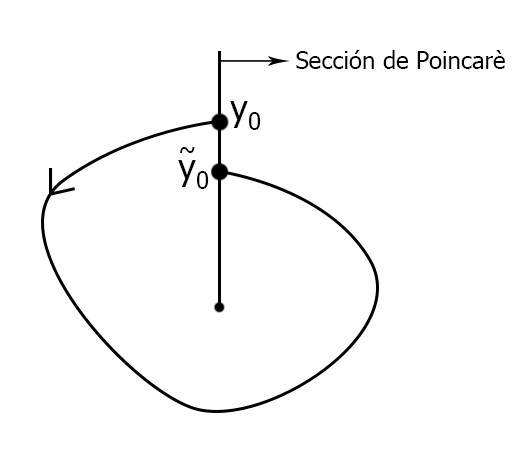
\includegraphics[width=0.8\textwidth]{aplipoincare2.jpg}
		\caption{Punto $y_0$ y su imagen $\tilde{y_0}$ mediante la Aplicación de Poincaré. Esta órbita no es periódica}
		\label{fig:aplipoincare2}
	\end{figure}\smallskip
	
\noindent Como vemos en la \fref{fig:aplipoincare2} la dinámica de estudio sería; establecer un punto $y_0$ mediente las condiciones iniciales de nuestro sistema, establecer una sección de Poincaré que corte a la curva solución y por último ver como avanza dicha curva en el tiempo esperando a que corte de nuevo a la sección de Poincaré, para que esto ocurra se debe cumplir una serie de condiciones en el sistema que ahora no presentaremos. Finalmente si la órbita vuelve a cortar en el mismo punto $y_0=\tilde{y_0}$ diremos que dicha órbita es periódica. 
	\newpage
	
	En este trabajo hablaremos de la \textit{\textbf{Semi-Aplicación de Poincarè}}, es decir, analizaremos una de las dos mitades de la orbita. Esto lo haremos ya que como nuestro estudio es de un sistema a trozos \eref{eq:lienardrl}, \eref{eq:lienardrlgr} ya tenemos una separación en la recta $x=0$ la cual usaremos de sección de Poincaré, y como a la izquierda y a la derecha de dicha sección tenemos sistemas diferentes debemos estudiarlos de manera independiente.
	
	\begin{figure}[h]
		\centering
		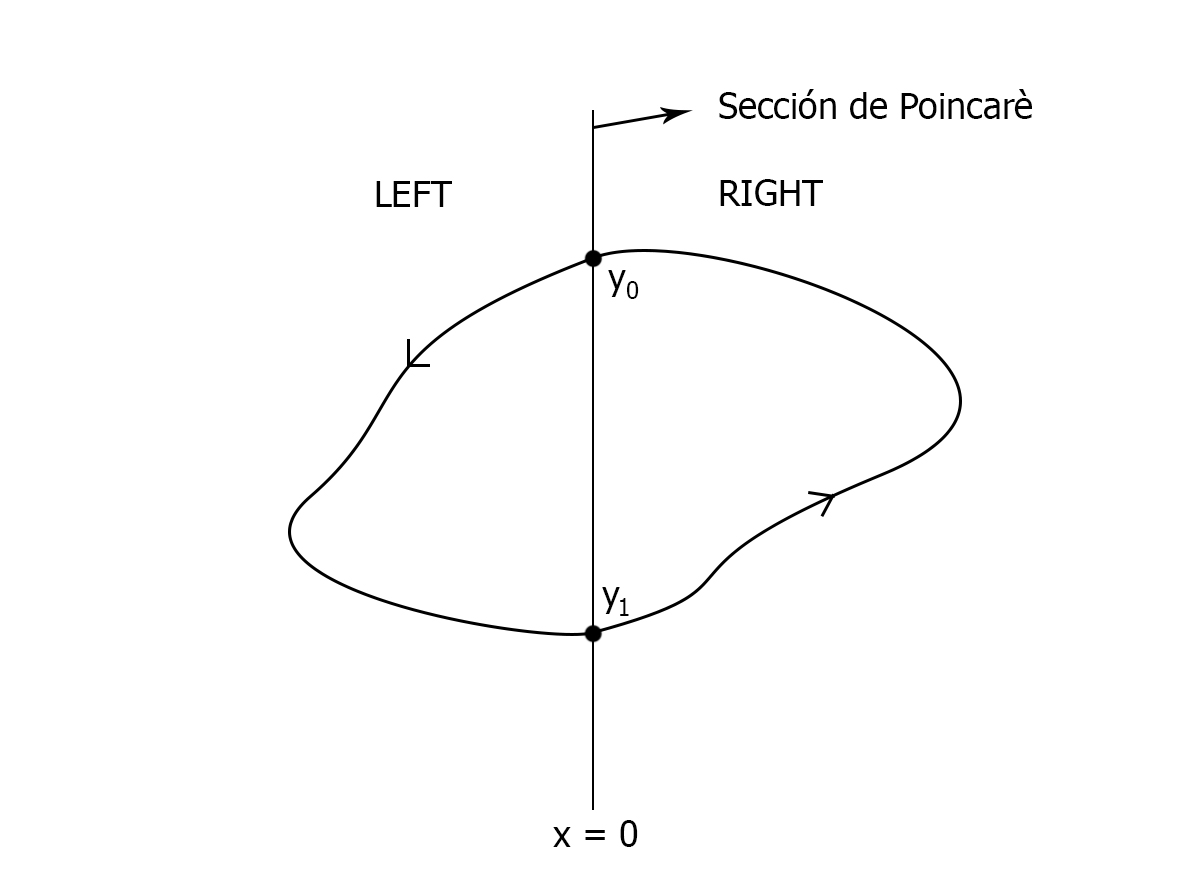
\includegraphics[width=0.9\textwidth]{poincaLR.jpg}
		\caption{Semiaplicación derecha e izquierda las cuales forman una órbita periódica}
		\label{fig:poincaLR}
	\end{figure}\smallskip
	
	Tendremos un punto de corte $y_0$ de nuestra órbita solución en la sección de Poincarè y buscaremos el siguiente punto de corte $y_1$ mediante la semiaplicación izquierda, finalmente mediante la semiaplicación derecha comprobamos si la órbita vuelve a cortar a la sección de Poincarè en el mismo punto $y_0$ (órbita periódica, ver \fref{fig:poincaLR}) o si no corta en el mismo punto $y_0$ (órbita no periódica).
	
	\vspace{0.5cm}Para la semiaplicación de Poincarè consideraremos el sistema \eref{eq:edo2}, que mediante los cambios de variable adeacuados podemos escribir en forma canónica de Lienard como ya hemos visto a lo largo de la Sección \ref{sistrobiz}. En dicha sección se hace para un sistema a trozos, pero para esta parte consideraremos un único sistema, que puede ser el derecho o el izquierdo, eso no nos importa ahora mismo por lo que la nomenclatura que usaremos en esta sección para dicho sistema será:
	
		\begin{equation}
		\label{eq:lienardsolo}
		\begin{pmatrix*}[r]
			\dot{x}\\ \dot{y}
		\end{pmatrix*}= \begin{pmatrix*}[r]
			T & -1 \\ D & 0
		\end{pmatrix*} \begin{pmatrix*}[r]
			x \\ y
		\end{pmatrix*}+\begin{pmatrix*}[c]
			0 \\ a
		\end{pmatrix*}
	\end{equation}\smallskip
	\newpage
	
	Definiendo la sección de Poincaré como $\varSigma=\left\{(x,y)^T\in \mathbb{R}^2:x=0\right\}$ donde nos referiremos con $\varSigma^L$ a la zona izquierda de la sección y $\varSigma^R$ a la zona derecha de la sección (recordemos que los índices R y L harán alusión a las zonas derecha e izquierda). Si evaluamos la primera ecuación de \eref{eq:lienardsolo} en la sección de Poincarè que hemos definido $\varSigma$ tenemos $\dot{x}|_{\varSigma}=-y$, pudiéndose deducir el sentido de la órbita:
	
	\begin{itemize}
		\item La órbita va de $\varSigma^L$ a $\varSigma^R$ para $y<0$
		\item La órbita va de $\varSigma^R$ a $\varSigma^L$ para $y>0$
	\end{itemize}
	
	Asumiremos $a^2+D^2\neq0$ ya que de no ser así curva solución no cortaría de nuevo a $\varSigma$. Esto se puede deducir estudiando la segunda ecuación del sistema \eref{eq:lienardsolo} para el caso contrario $a=D=0 \longrightarrow \dot{y}=Dx+a=0$.
	
	\vspace{0.5cm}Vamos a centrarnos en la zona izquierda de la sección de Poicaré $\varSigma^L$, la cual se define de la siguiente manera:

	\begin{definicion}
		\label{def6}
		Consideraremos el punto $(0,y_0)\in \varSigma$ con $y_0\geq0$ y tomaremos como solución del sistema \eref{eq:lienardsolo} para cada instante de tiempo $\phi(t)=(\phi_1(t),\phi_2(t))$, que para el instante inicial $t=0$ cumple que $\phi(0)=(0,y_0)$. Si existe un valor de tiempo $\tau>0$ para el que se cumple $\phi_1(\tau)=0$ y $\phi_1(t)<0$ para todo $t\in(0,\tau)$ decimos que la imagen de $y_0$ por la semiaplicación izquierda de Poincaré $P_L(y_0)=y_1=\phi_2(\tau)\leq0$. El valor de tiempo $\tau$ se denomina semi-tiempo de vuelo izquierdo.
	\end{definicion}
	
	\begin{figure}[h]
		\centering
		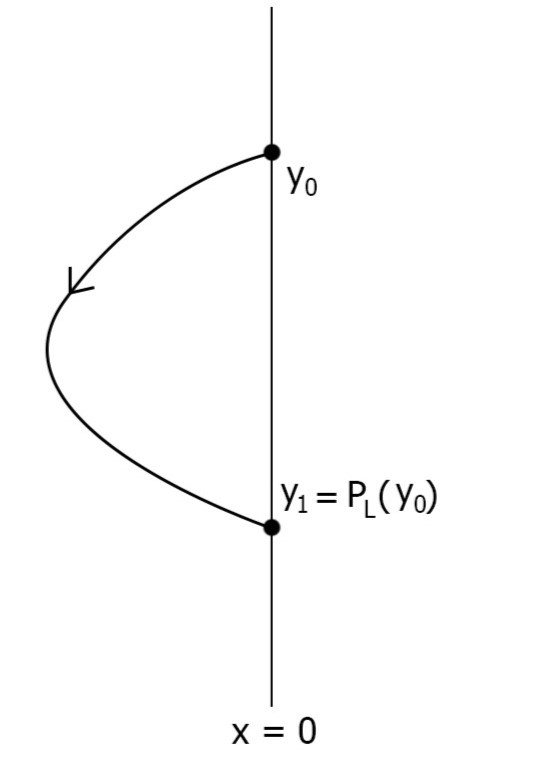
\includegraphics[width=0.6\textwidth]{semiL.jpg}
		\caption{ Semiaplicación de Poincaré Izquierda}
		\label{fig:semiL}
	\end{figure}\smallskip
	\newpage
	
	\textit{\textcolor{red}{Añadir $P(0)=0$? no entiendo muy bien esa parte (articulo caracterizacion integral)}}
	
	
	La definción de la semiaplicación de Poincaré derecha es equivalente a la izquierda ya que el sistema \eref{eq:lienardsolo} no varia sus propiedades cuando se le aplica el cambio de variable $(x,y,a)\longleftrightarrow(-x,-y,-a)$.
	
	
	\vspace{0.5cm} La definición \ref{def6} invita a estudiar la dinámica del sistema mediante integración, este es el método clásico, el cual conlleva una gran cantidad de posibles casos debidos a las particularidades de las matrices características para cada sistema que estudiemos. Casos que deben estudiarse uno a uno y aplicando diferentes herramientas para cada uno de ellos, lo cual se traduce en gran dificultad para el estudio y obtención de aparentemente distintos resultados para el mismo sistema dependiendo de que herramienta matemática usemos para solucionarlo. Para arreglar esta problemática usaremos la caracterización integral de la semiaplicación de Poincaré, ver \textit{\textcolor{red}{(articulo caracterizacion integral)}}, la cual presentaremos en la sección \ref{sec41}.
	\newpage
	
	
	
	\section{Caracterización integral de la semi-aplicacion de Poincare}
	\label{sec41}
	
	No nos olvidemos que al fin y al cabo lo que tenemos en el sistema \eref{eq:lienardrlgr} sigue siendo un sistema de dos ecuaciones con dos incógnitas a cada lado de la sección $\varSigma \rightarrow x=0$. Como ya dije en la sección de \ref{sec:sislinplanos} no vamos a solucionar estos sistemas de la manera clásica. Lo que nos interesa es que dado un punto $y_0$ encontremos su correspondiente imagen mediante la semiaplicacion de poincaré izquierda $y_1=P_L(y_0)$. Y como queremos una orbita periódica lo que haremos para cerrar dicha órbita es encontrar la imagen mediante la semiaplicacion de poincaré derecha con el tiempo invertido $y_1=P_R^{-1}(y_0)$ haciendo que las imágenes $y_1$ de cada semiaplicación sean la misma y por tanto cerrando la órbita. Ojo, estamos buscando puntos, no estudiamos las órbitas por eso puede parecer que vamos en sentido contrario al tiempo en la semiaplicacion derecha, pero no olvidemos que las órbitas y sus sentidos no nos interesa, solo los puntos $y_0$ e $y_1$ que hagan que aparezca una orbita periodica. Lo hacemos de esta manera por que es la mas sencilla de solucionar, el trabajo se reduce a coger un punto $y_0$, hallar sus semiaplicaciones izquierda y derecha y comprobar si cortan a la sección de Poincaré $\varSigma$ en el mismo punto $y_1$. 
	\textit{\textcolor{red}{Reescribir todo este párrafo. Añadir idea que la abstraccion de la órbita y del tiempo es gracias a la caracterizacion y no a la propia semiaplicacion(foto a 0.8)}}
	
	 \begin{figure}[h]
		\centering
		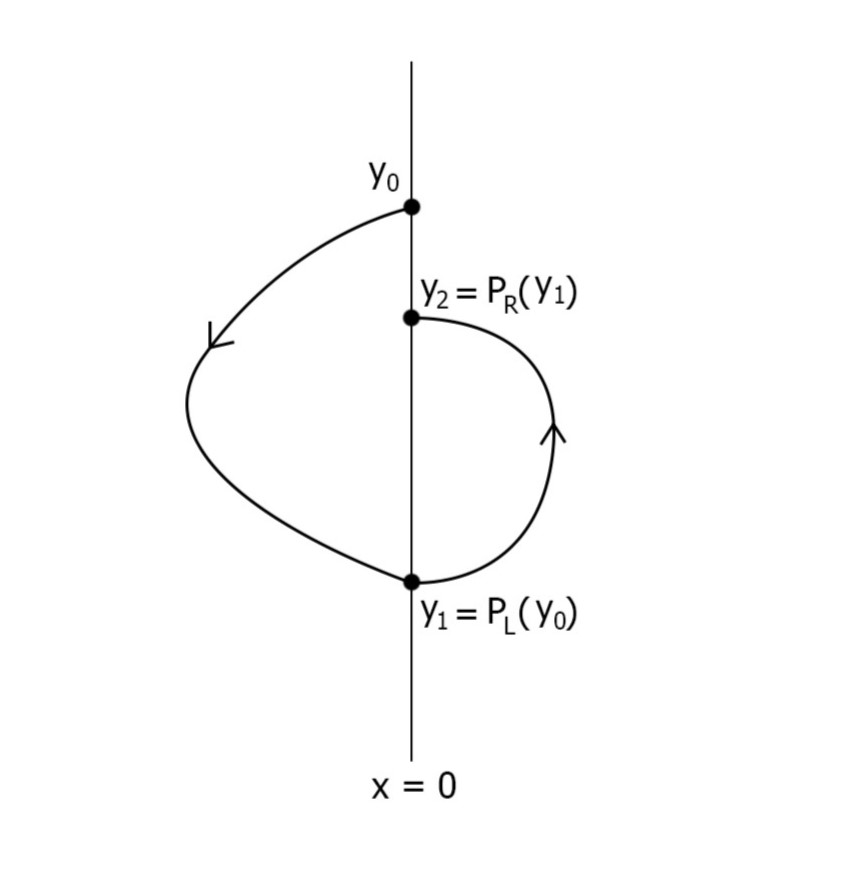
\includegraphics[width=0.7\textwidth]{aplipoincareLR.jpg}
		\caption{Semiaplicaciones izquierda y derecha del punto $y_0$ con diferentes imagenes $y_1$,$y_2$.}
		\label{fig:aplipoincareLR}
	\end{figure}\smallskip
	\newpage
	
	 \begin{figure}[h]
		\centering
		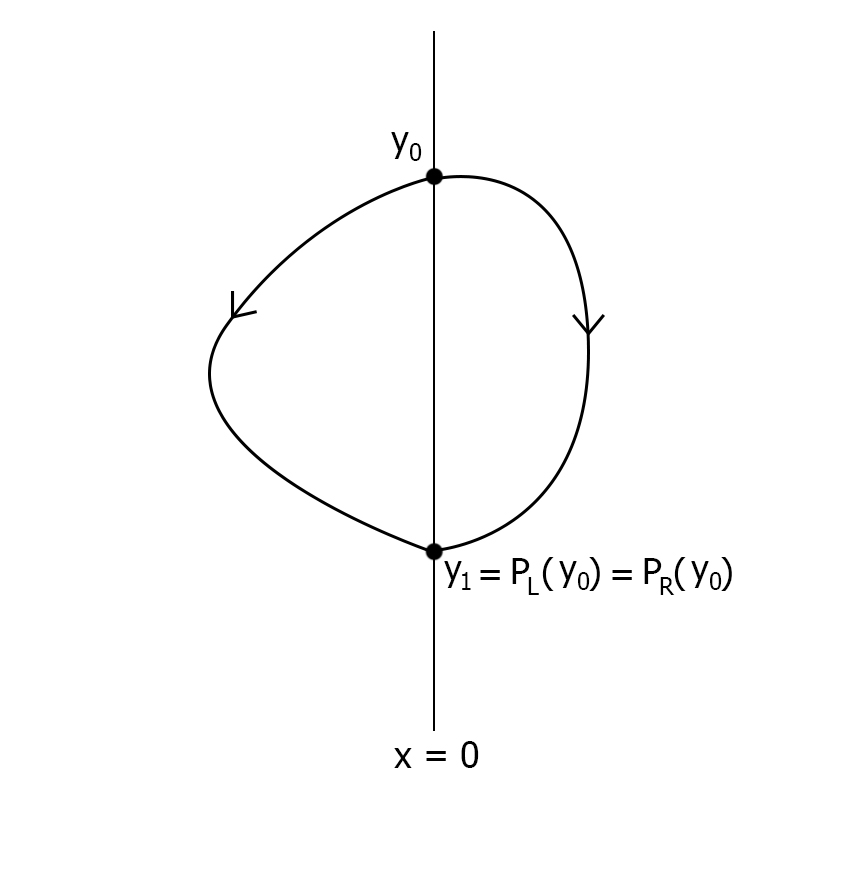
\includegraphics[width=0.8\textwidth]{aplipoincareLR - copia.jpg}
		\caption{Semiaplicaciones izquierda y derecha del punto $y_0$ con misma imagen $y_1$ y por lo tanto formando una órbita periódica.}
		\label{fig:aplipoincareLR - copia}
	\end{figure}\smallskip
	    
	Para hallar esta igualdad en las semiaplicaciones derecha e izquierda haremos uso de una herramienta presentada en \textit{\textcolor{red}{citar caracterizacion integral}}. Se trata de realizar una caracterización integral de la semiaplicacón de poincaré. 
		
	\vspace{0.5cm} Primeramente debemos presentar el \textit{\textbf{Valor Principal de Cauchy}} $\left(PV\right)$, ya que se utiliza en la caraterización integral. El valor principal de Cauchy es una herramienta matematica muy usada en análisis complejo y teoria de funciones para definir una integral principal en casos de discontinuidades evitables en el plano complejo. Consideremos un inntervalo $[a,b]$ que contiene al origen y una funcion $f$ continua en $[a,b],\left\{0\right\}$, el Valor Principal de Cauchy se define como:

	\begin{equation}
		\scalebox{1.2}{$\displaystyle
		 PV\left\{\int_{a}^{b}f(x)dx\right\}= \lim_{\epsilon \to 0^+}\left(
		\int_{a}^{-\epsilon}f(x)dx \; + \; 
		\int_{+\epsilon}^{b}f(x)dx
		\right)
		$}
	\end{equation}\smallskip
	\newpage
	
	\vspace{0.5cm} Vamos a pasar a presentar la ecuacion de la caracterizacion integral y sus propiedades.
	
	\vspace{0.5cm}\noindent Caracterización integral de la semiaplicación de Poincaré izquierda:
	\begin{equation}
		\label{eq:caracl}
		\scalebox{1.2}{$\displaystyle
		PV\left\{\int_{y_1}^{y_0}\frac{-y}{D_Ly^2-aT_Ly+a^2}dy\right\}=\frac{k_L\pi T_L}{D_L\sqrt{aD_L-T_L^2}}
		$}
	\end{equation}\smallskip
	
	\vspace{0.5cm}\noindent Caracterización integral de la semiaplicación de Poincaré derecha:
	\begin{equation}
		\label{eq:caracr}
		\scalebox{1.2}{$\displaystyle
			PV\left\{\int_{y_1}^{y_0}\frac{-y}{D_Ry^2-aT_Ry+a^2}dy\right\}=\frac{-k_R\pi T_R}{D_L\sqrt{aD_L-T_L^2}}
			$}
	\end{equation}\smallskip
	
	\noindent donde los parámetros $D_L,T_L,D_R,T_R,a$ son los correspondientes al sistema a trozos \eref{eq:lienardrl} e $y_0$ corresponde al primer punto de corte con la seccion de Poincaré $\varSigma$ e $y_1$ la imagen de $y_0$ mediante la semiaplicaciones de Poincaré, ver \fref{fig:aplipoincareLR}. Como se puede ver en \eref{eq:caracl} y \eref{eq:caracr} el valor principal de cauchy solo lo usaremos en el caso de $a=0$ ya que la integral se vuelve impropia divergente, en el caso de $a\neq0$ el valor principal de cauchy es directamente el valor de la integral. Los parámetros $k_L,k_R$ tomarán los siguientes valores en función del signo de $a$ y de en qué zona estemos de la sección de Poincaré
	
	\vspace{0.5cm}\noindent Zona izquierda:
	\begin{itemize}
		\item $k_L=0 \qquad si \quad a_L>0$
		\item $k_L=1 \qquad si \quad a_L=0$
		\item $k_L=2 \qquad si \quad a_L<0$
	\end{itemize}\smallskip
	
		\noindent Zona derecha:
	\begin{itemize}
		\item $k_R=0 \qquad si \quad a_R<0$
		\item $k_R=1 \qquad si \quad a_R=0$
		\item $k_R=2 \qquad si \quad a_R>0$
	\end{itemize}\smallskip
	\newpage
	
	Lo unico que diferencia a las ecuaciones \eref{eq:caracl} y \eref{eq:caracr} es el signo menos del segundo término, el cual se debe al sentido del tiempo. Como ya comentamos antes el sentido lógico en nuestro caso para la semiaplicación derecha sería ir de $y_1$ a $y_0$ lo cual se denominaría $y_0=P_R(y_1)$ y en este caso el signo del segundo termino de la caracterización sería positivo, pero nosotros estamos calculando la semiaplicacion derecha de $y_0$ a $y_1$ lo que es $y_1=P_R^{-1}(y_0)$, por ello aparece el signo negativo en el segundo termino de la caracterización integral de la semiaplicación derecha \eref{eq:caracr}. Aunque realmente este signo negativo no nos importa, como he dicho el punto de equilibrio de nuestro sistema estará en la zona izquierda por lo que $k_R=0$, ver la anterior lista, así que el segundo término valdrá cero para la semiaplicacion derecha.\textit{\textcolor{red}{preguntar por este párrafo completo, si en nuestro estudio kr=0 siempre y como meter las imganes de matlab sin que sean figuras}}
	
	\vspace{0.5cm} Vamos a ver algunos ejemplos de la caracterizacion integral de la semiaplicación de Poincaré en MATLAB para entender un poco mejor la estrategia de busqueda de la oscilación periódica.
	
	\begin{figure}[h]
		\centering
		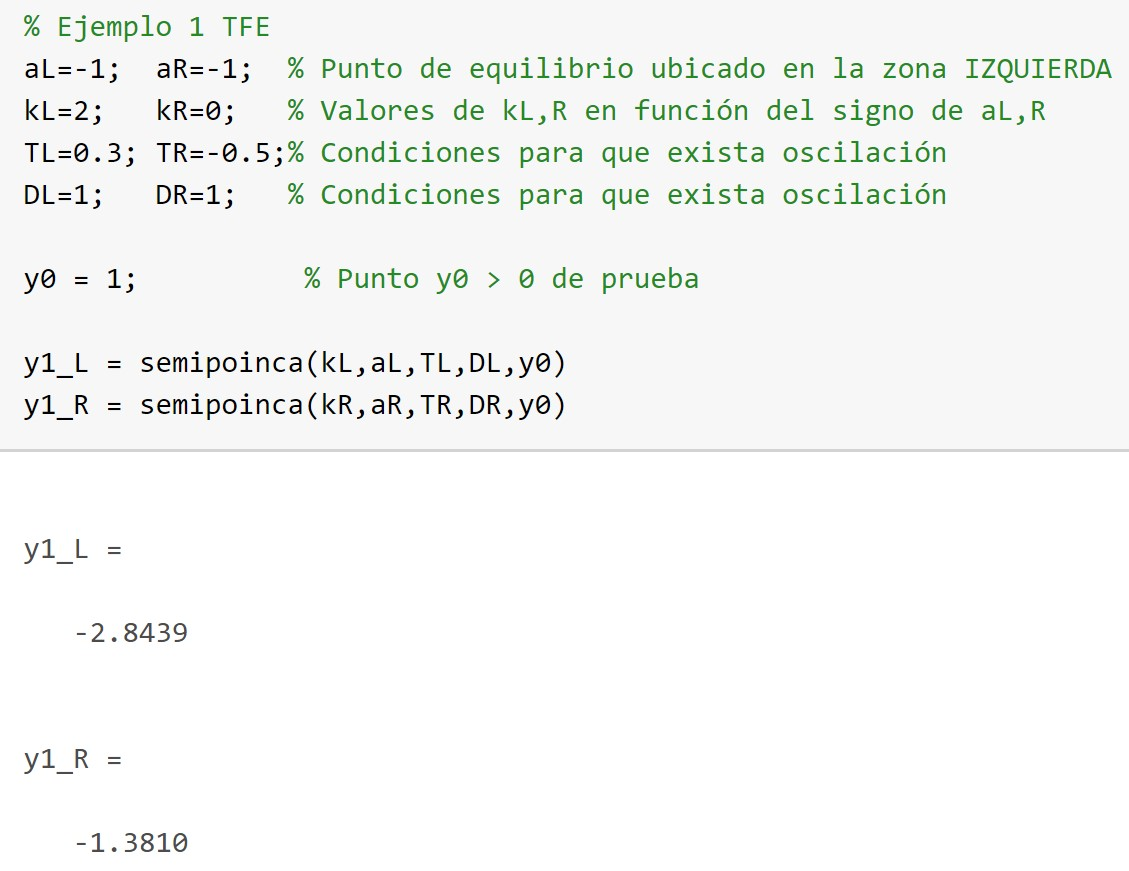
\includegraphics[width=1\textwidth]{ejem1.jpg}
		\caption{Semiaplicaciones izquierda y derecha de un punto de ejemplo $y_0$}
		\label{fig:ejem1}
	\end{figure}\smallskip
	\newpage
	
		\begin{figure}[h]
		\centering
		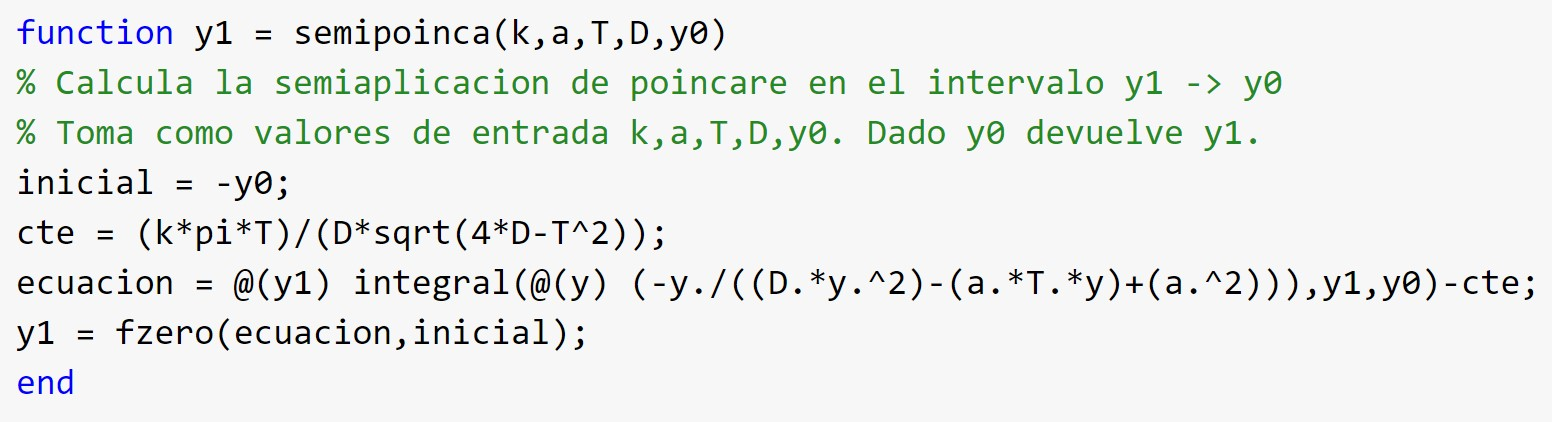
\includegraphics[width=1\textwidth]{ejem1_1.jpg}
		\caption{Función usada en \fref{fig:ejem1} que hace el cálculo de la caracterización}
		\label{fig:ejem1_1}
	\end{figure}\smallskip
	
	La función de la \fref{fig:ejem1_1} es la aplicación directa de la caracterización integral en MATLAB. Veamos que se sestá haciendo:
	
	\vspace{0.5cm}\noindent Primero vamos a reordenar la función de la caracterización izquierda \eref{eq:caracl}:
	
	\begin{equation}
			\label{eq:eje1}
		\scalebox{1.2}{$\displaystyle
		\begin{gathered}
			\int_{y_1}^{y_0}\frac{-y}{D_Ly^2-aT_Ly+a^2}dy=\frac{k_L\pi T_L}{D_L\sqrt{aD_L-T_L^2}} \\[2mm]
			\int_{y_1}^{y_0}\frac{-y}{D_Ly^2-aT_Ly+a^2}dy-\frac{k_L\pi T_L}{D_L\sqrt{aD_L-T_L^2}}=0
		\end{gathered}
			$}
	\end{equation}\smallskip
	
	\noindent como vemos en \fref{fig:ejem1_1} tenemos como parámetros de entrada $k,a,T,D,y_0$ y como parámetro de salida $y_1$, por lo que la ecuación \eref{eq:eje1} se puede reducir a:
	
	\begin{equation}
		\label{eq:eje2}
		\scalebox{1.2}{$\displaystyle
				f(y_1)-cte=0
			$}
	\end{equation}\smallskip
	
	\noindent de manera más genérica aún, el término constante lo podemos considerar dentro de $f(y_1)$ por lo que
	
		\begin{equation}
		\label{eq:eje3}
		\scalebox{1.2}{$\displaystyle
				f(y_1)=0
			$}
	\end{equation}\smallskip
	
	\noindent finalmente la ecuación \eref{eq:eje3} ya está en la forma adecuada para resolverla con la función \textit{fzero} de MATLAB, introduciendo como punto inicial $-y_0$, ver \fref{fig:ejem1_1}. La función \textit{fzero} resuelve de manera numérica una ecuación tipo $f(x)=0$ con $x_0$ como punto inicial.
	
	\vspace{0.5cm}\noindent El código de la \fref{fig:ejem1} simplemente describe las características de los sistemas a la izquierda y a la derecha, describe un punto de prueba $y_0=1$ y llama a la función \textit{semipoinca} para calcular las semiaplicaciones derecha e izquierda. Como se ve obtenemos valores diferentes, de hecho la semiaplicación izquierda tiene un valor mas grande que la derecha, gráficamente podría ser perfectamente lo representado en la \fref{fig:aplipoincareLR}.
	\newpage
	
	Vale, no hemos consguido que las imágenes $y_1$ fueran las mismas, por lo que ahora lo que haríamos sería probar con otro punto $y_0$ y volver a comprobar si se cumple que $y_{1_L}=y_{1_R}$. Obviamente no lo vamos a hacer de manera manual, tenemos suficientes herramientas para hacerlo. Como hemos visto para usar \textit{fzero} necesitamos un punto inicial, sin entrar mucho en detalle de resolución numérica \textit{\textcolor{red}{hablar de como funciona fzero y de porque elegir el punto cerca de la solucion es útil?}}, basicamente este punto cuanto más cercano a la solución lo eligamos mas fiable y rápida será dicha solución, por ello vamos a representar de manera gráfica las semiaplicaciones izquierda y derecha para un intervalo de puntos $y_0 \in [0\;\;10]$ y veamos si encontramos un punto de corte que nos indique que para un $y_0$ las imágenes son las mismas
	
	\begin{figure}[h]
		\centering
		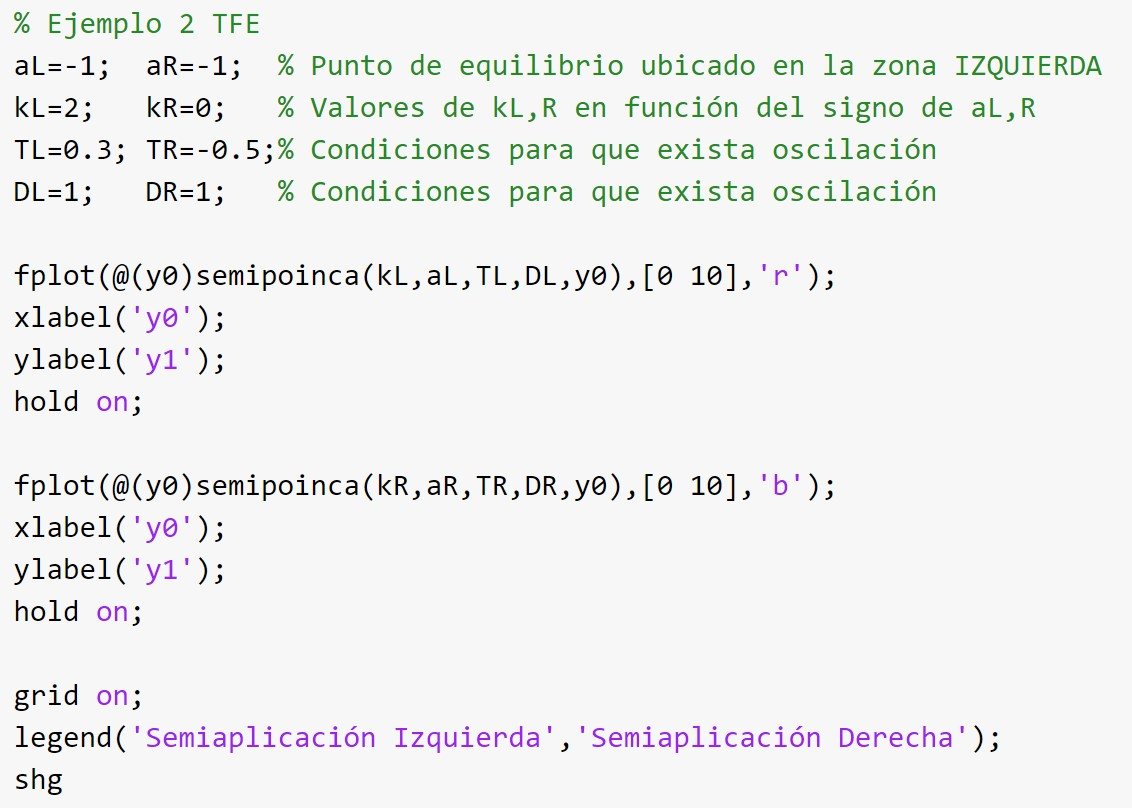
\includegraphics[width=1\textwidth]{ejem2.jpg}
		\caption{Código para generar las gráficas de las semiaplicaciones izquierda y derecha}
		\label{fig:ejem2}
	\end{figure}\smallskip
	
	En este caso usamos \textit{fplot} la cual va evaluando la función probando continuamente con valores de $y_0$ desde cero hasta diez, se pintará de rojo la semiaplicación izquierda y de azul la semiaplicación derecha 
	\newpage
	
	\begin{figure}[h]
		\centering
		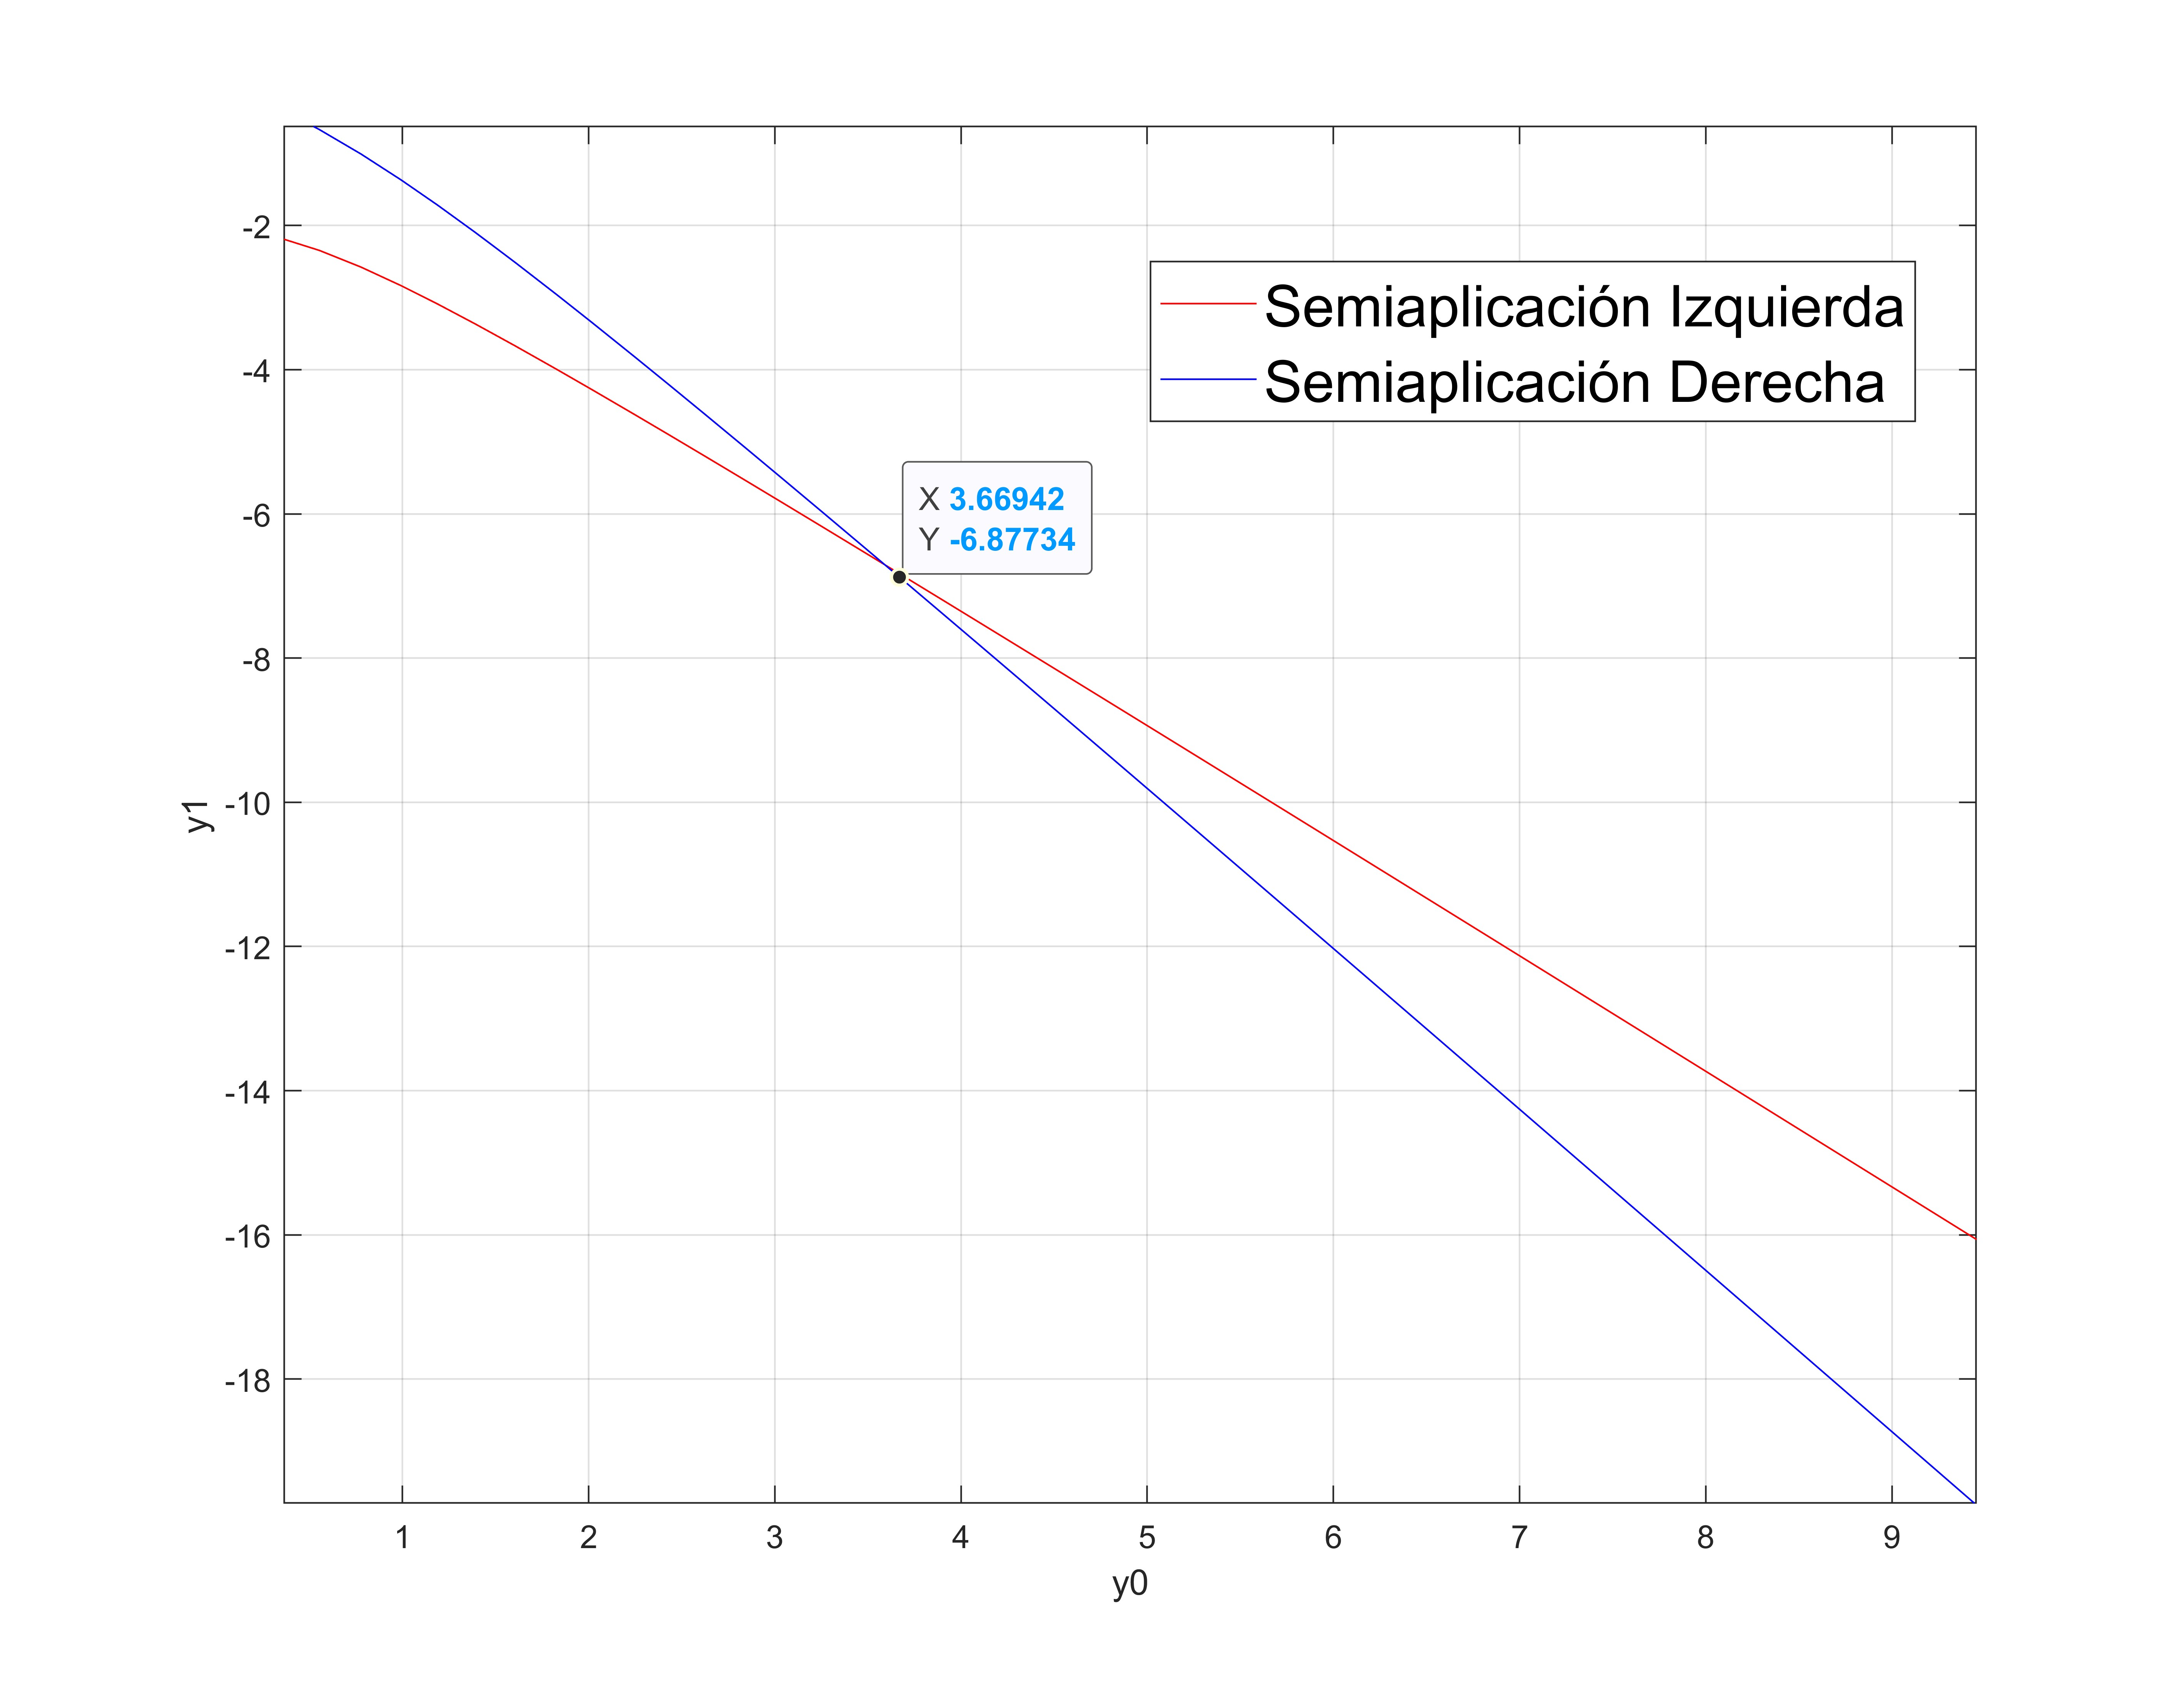
\includegraphics[width=1\textwidth]{ejem2_2.jpg}
		\caption{Gráfica obtenida de las semiapliaciones izquierda y derecha}
		\label{fig:ejem2_2}
	\end{figure}\smallskip
	
	Como vemos en la \fref{fig:ejem2_2} efectivamente se cortan las gráficas, simplemente pinchando más o menos en el punto de corte vemos que las semiaplicaciones izquierda y derecha tendrán la misma imagen $y_1\approx-6.87734$ cuando $y_0\approx3.66942$.
	\newpage
	Ya tenemos el punto que estará muy cercano a la solución que buscamos, ahora vamos a calcularla exactamente de manera numérica usando \textit{fsolve} que nos permite solucionar los mismos casos que \textit{fzero} y para más de una variable. Pero primero hay que escribir correctamente la función en MATLAB
	
		
	\begin{figure}[h]
		\centering
		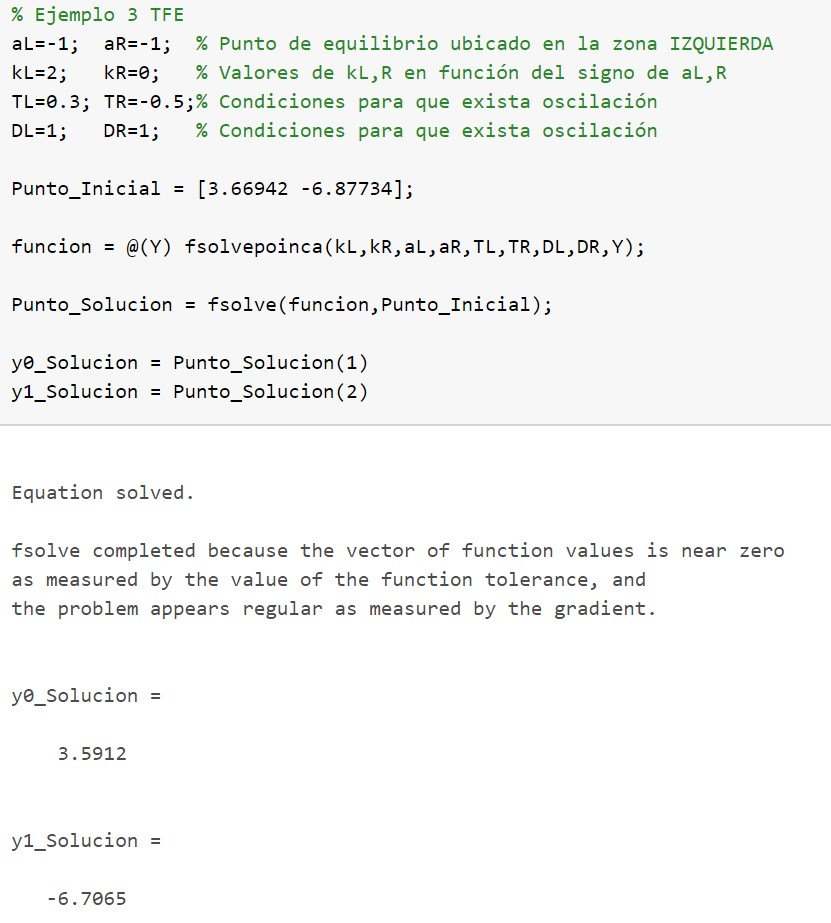
\includegraphics[width=1\textwidth]{ejem3.jpg}
		\caption{Código para obtener los valores exactos de $y_0$ e $y_1$ para los que hay un órbita periódica}
		\label{fig:ejem3}
	\end{figure}\smallskip
	
	Efectivamente como se puede ver en la \fref{fig:ejem3} los valores que hemos obtenidos son muy parecidos a los que vimos en la \fref{fig:ejem2_2}. Podemos decir entonces, que para el sistema que hemos estudiado tenemos una oscilación periódica que va desde $y_0=3.5912\;$ hasta $\; y_1=-6.7065$. Veamos la función \textit{fsolvepoinca} la cual es llamada en el codigo anterior
	\newpage
	\begin{figure}[h]
		\centering
		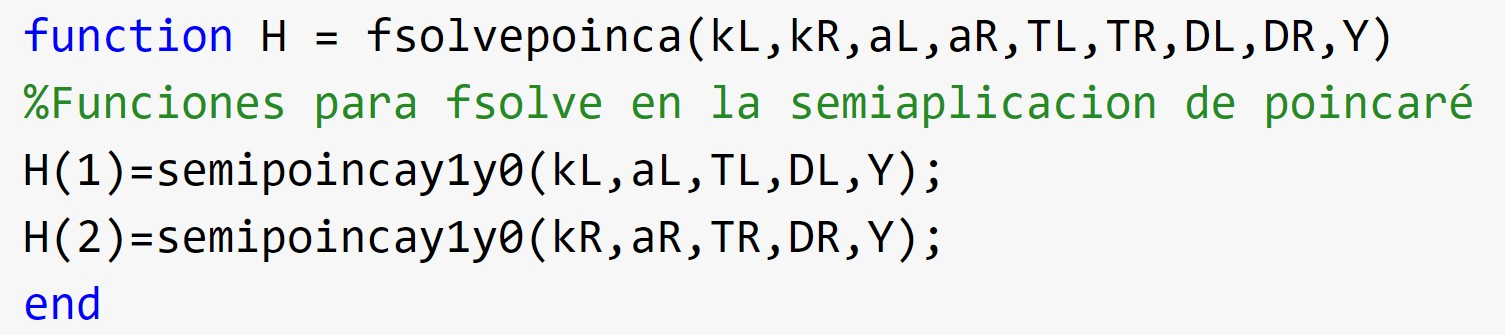
\includegraphics[width=1\textwidth]{ejem3_1.jpg}
		\caption{Función usada para separar las caracteristicas izquierda, derecha y llama la funcion \textit{semipoincay1y0} la cual se encarga de calcular la semiaplicacion}
		\label{fig:ejem3_1}
	\end{figure}\smallskip
	
	Como vemos en \fref{fig:ejem3} se llama a una función \textit{fsolvepoinca}, la cual vemos en la \fref{fig:ejem3_1}. Los parámetros de entrada de \textit{fsolvepoinca} son las caracteristicas de los sistemas de la derecha y de la izquierda $k,a,T,D$ además de un vector de dos componentes $Y$, este vector contiene el punto inicial, que como vemos en la \fref{fig:ejem3} le hemos asignado el punto de corte que más o menos obtuvimos viendo la gráfica de la \fref{fig:ejem2_2}.
	\vspace{0.5cm}
	\begin{figure}[h]
		\centering
		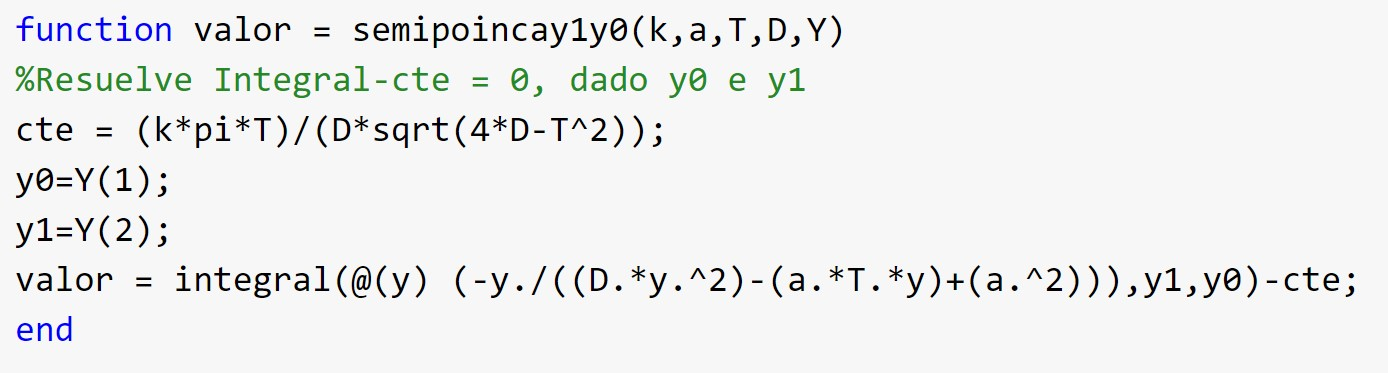
\includegraphics[width=1\textwidth]{ejem3_2.jpg}
		\caption{}
		\label{fig:ejem3_2}
	\end{figure}\smallskip
	
	En este caso queremos evaluar la ecuación \eref{eq:eje1} ya que estamos aportando valor a todos los parámetros $y_0,y_1,k,a,T,D$. Por ello con la función \textit{semipoincay1y0}, ver \fref{fig:ejem3_2}, se está evaluando:
	
	\begin{equation}
		\label{eq:eje4}
		\scalebox{1.2}{$\displaystyle
			f(y)=integral - cte
			$}
	\end{equation}\smallskip
	
	\noindent aportando como punto incial el vector $Y=\left[ y_0 \; y_1 \right]$. La función \textit{fsolve} del código de la \fref{fig:ejem3} buscará el punto, valores $\left(y_0\; y_1\right)$, en que las curvas de las semiaplicaciones derecha e izquierda se cortan.
	
	\chapter{Bifurcación Foco-Centro-Ciclo Límite}
	La forma de que aparezca una oscilación en un sistema dinámico es mediante bifurcaciones. Las bifurcaciones aparecen cuadno variamos de manera progresiva un parámetro del sistema, llamado parámetro de control. Esta variación puede producir una bifurcación debido a la creación o destrucción de un punto de equilibrio (bifurcación Hopf-Like) o cambiando la estabilidad del sistema mediante la variación de la traza $T$, este será nuestro caso. A esta bifurcación producida por la variación de la traza del sistema se le llama \textbf{Foco-Centro-Ciclo Límite}, ver \textit{\textcolor{red}{citar articulo de ponce donde se da este nombre y se presenta}}, pero antes de presentarla vamos a hacer el análisis del punto de equilibrio y la estabilidad del sistema que estamos estudiando y el concepto de ciclo-límite para posteriormente ver como generar esta bifurcación en nuestro circuito.
	
		\vspace{0.5cm}Para hacer el análisis del punto de equilibrio y de la estabilidad primero recordemos el sistema que tenemos. Nosotros estamos estudiando un sistema, dinámico, autónomo, lineal y continuo a trozos bizonal en forma canónica de Lienard, recordar el sistema \eref{eq:lienardrl}, \eref{eq:lienardrlgr}.
		
		\vspace{0.5cm}Podemos obtener los puntos de equilibrio de cada una de las zonas igualando a cero el sistema, por ejemplo para la zona izquierda tenemos:
		
		\begin{equation*}
			\begin{pmatrix*}[r]
				0\\ 0
			\end{pmatrix*}= \begin{pmatrix*}[r]
				T_L & -1 \\ D_L & 0
			\end{pmatrix*} \begin{pmatrix*}[r]
				x \\ y
			\end{pmatrix*}+\begin{pmatrix*}[r]
				0 \\ a
			\end{pmatrix*}
		\end{equation*}\smallskip
		
		\begin{equation}
			\label{eqpointL}
			\left\{
			\begin{aligned}
				T_Lx-y=0\\
				D_Lx-a=0
			\end{aligned}
			\right. \quad \longrightarrow \left( \overline{x},\overline{y} \right)=\left( \frac{a}{D_L},\frac{aT_L}{D_L} \right)
		\end{equation}\smallskip
		
		Análogamente para la zona derecha tendríamos el punto de equilibrio:
		
		\begin{equation}
			\label{eqpointR}
			\left( \overline{x},\overline{y} \right)=\left( \frac{a}{D_R},\frac{aT_R}{D_R} \right)
		\end{equation}\smallskip
		\newpage
		Como podemos comprobar el valor de $a$, que como vimos en \eref{eq:sgn} nos indica el signo, nos está diciendo donde se encuentra el punto de equilibrio respecto a la recta de separación:
		
		\begin{figure}[h]
			\centering
			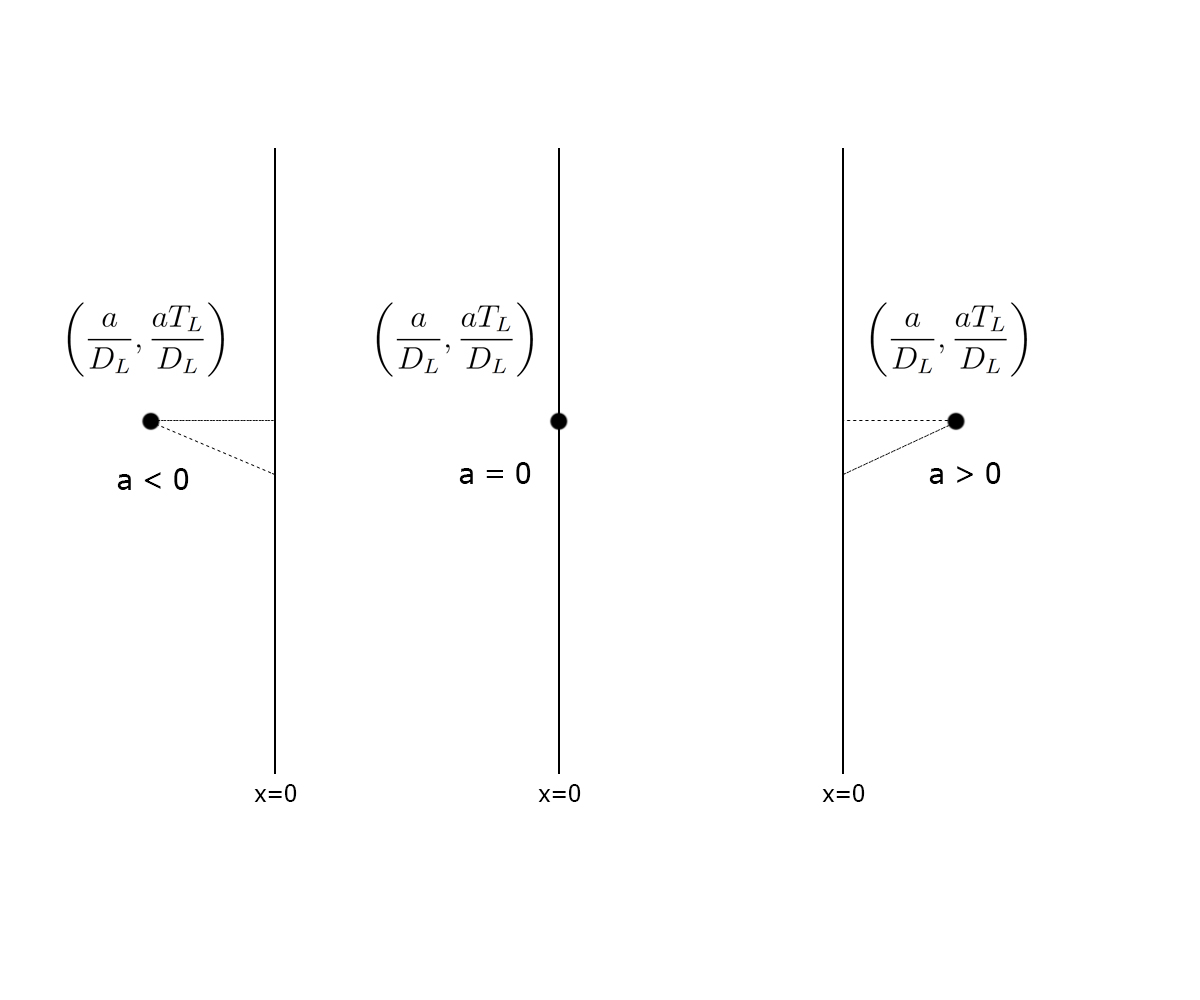
\includegraphics[width=1\textwidth]{punto.jpg}
			\caption{Posición del punto de equilibrio de la zona izquierda dependiendo del signo de $a$.}
			\label{fig:punto}
		\end{figure}\smallskip
		
		La posición del punto de equilibrio de la zona derecha es análoga a la de la zona izquierda, ver \fref{fig:punto}, pero en este trabajo nos centraremos en la zona izquierda únicamente. Mas adelante veremos como lo que ocurra en la zona derecha del plano de separación no nos afectará.
		
		\vspace{0.5cm} Una vez obtenido el punto de equilibrio podemos analizar la estabilidad como ya hicimos en \eref{eq:equilibrio}, veámoslo de nuevo con la nueva nomenclatura que hemos elegido. El polinomio característico de la zona izquierda sería:
		
		\begin{eqnarray}
			\label{eq:eqizq}
			\begin{aligned}
				P_{A_L}(\lambda)=&\lambda^2-tr(A_L)\lambda+det(A_L) \\[1mm]
				&\lambda^2-T_L\lambda+D_L=0 \\[2mm]
				\textit{Autovalores}\rightarrow \quad &\lambda=\frac{T_L\pm \sqrt{T_L^2-4\,D_L}}{2}
			\end{aligned}
		\end{eqnarray}\smallskip
		\newpage
		Como se puede ver el polinomio característico \eref{eq:eqizq} es análogo al del sistema \eref{eq:equilibrio} el cual ya analizamos, así que estaremos buscando:
		
		\begin{itemize}
			\item $T_L^2-4\,D_L<0\quad$ por lo que $\quad D_L>0$.
			\item $T_L<0\quad$ para tener un foco asíntoticamente estable.
			\item $T_L=0\quad$ para tener un centro.
			\item $T_L>0\quad$ para tener un foco asíntoticamente inestable.
		\end{itemize}\smallskip
		
		\vspace{0.5cm}Se puede ver que el cambio en la estabilidad del sistema lo produce un cambio en la traza, en nuestro caso la traza izquierda. Este cambio en la traza en nuestro sistema se traducirá en cambiar fisicamente el valor de alguna variable, haremos los ajustes necesarios para que este cambio en la traza se produzca cambiando la resistencia del circuito, ya que se podría hacer facilmente con un potenciometro.
		
		\vspace{0.5cm}El siguiente concepto que debemos conocer es el de \textbf{Ciclo-Límite}. Un Ciclo-Límite es una solución periódica del sistema la cual está aislada, es decir, no existen mas soluciones periódicas cercanas a ella en el plano de fases. Del mismo modo que los puntos de equilibrio pueden tener diferentes estabilidades, hay tres posibles estabilidades para un ciclo límite.\\[0.5cm]
		
		{\Large\textbullet\quad Ciclo-Límite Estable}\\[0.5cm]
		
		No importa si elegimos las condiciones iniciales dentro o fuera del Ciclo-Límite, las curvas solución tienden al Ciclo-Límite.
		
		\begin{figure}[h]
			\centering
			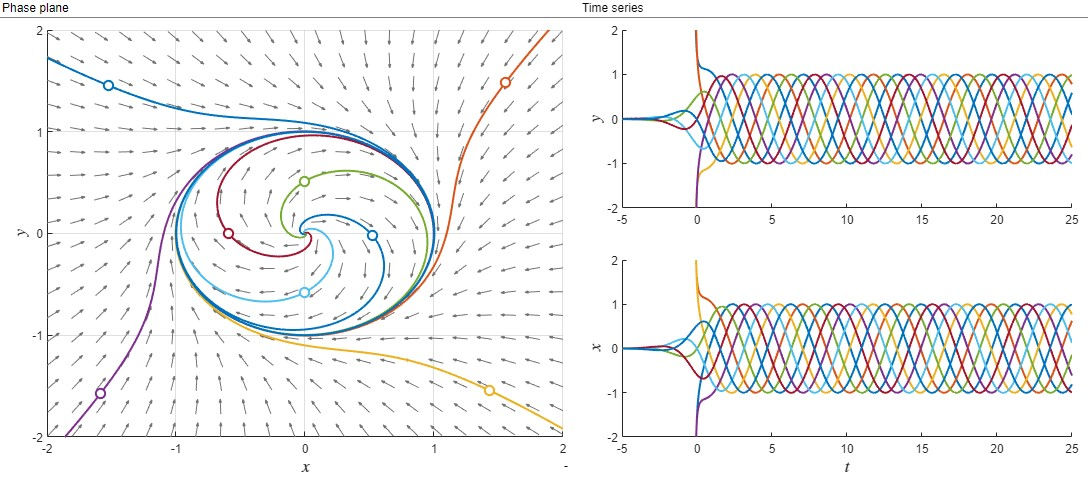
\includegraphics[width=1\textwidth]{cle.jpg}
			\caption{Ciclo-Límite Estable con sentido horario de giro}
			\label{fig:cle}
		\end{figure}\smallskip

	\newpage
		
	{\Large\textbullet\quad Ciclo-Límite Inestable}\\[0.5cm]
	
	Si elegimos las condiciones iniciales dentro del Ciclo-Límite, las curvas solución tienden a cero. Si elegimos las condiciones iniciales fuera del Ciclo-Límite, las curvas solución tienden a infinito.
	
	\begin{figure}[h]
		\centering
		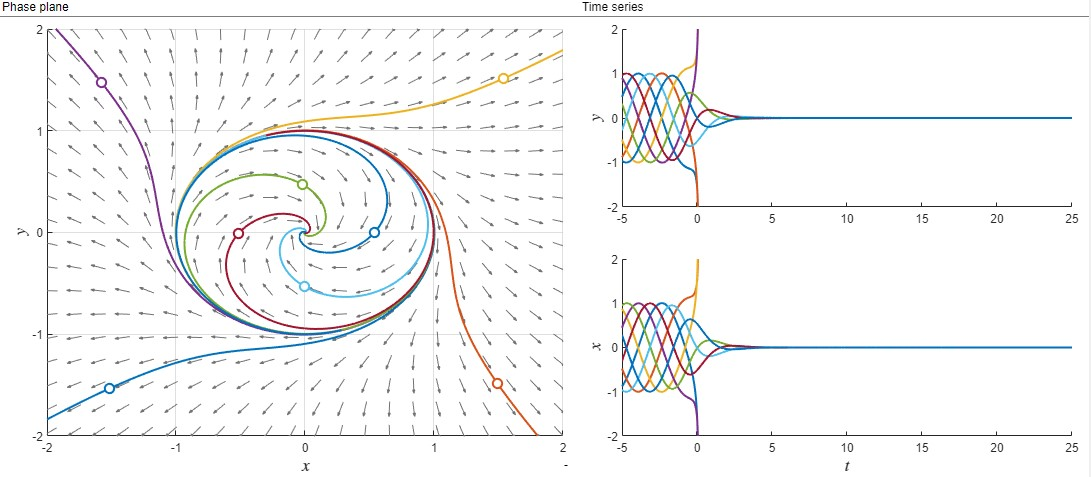
\includegraphics[width=1\textwidth]{cli.jpg}
		\caption{Ciclo-Límite Inestable con sentido horario de giro}
		\label{fig:cli}
	\end{figure}\smallskip
	
	\vspace{0.5cm}{\Large\textbullet\quad Ciclo-Límite Parcialmente Estable}\\[0.5cm]
	
	Si elegimos las condiciones iniciales dentro del Ciclo-Límite, las curvas solución tienden a cero. Si elegimos las condiciones iniciales fuera del Ciclo-Límite, las curvas solución tienden al Ciclo-Límite.
	
	\begin{figure}[h]
		\centering
		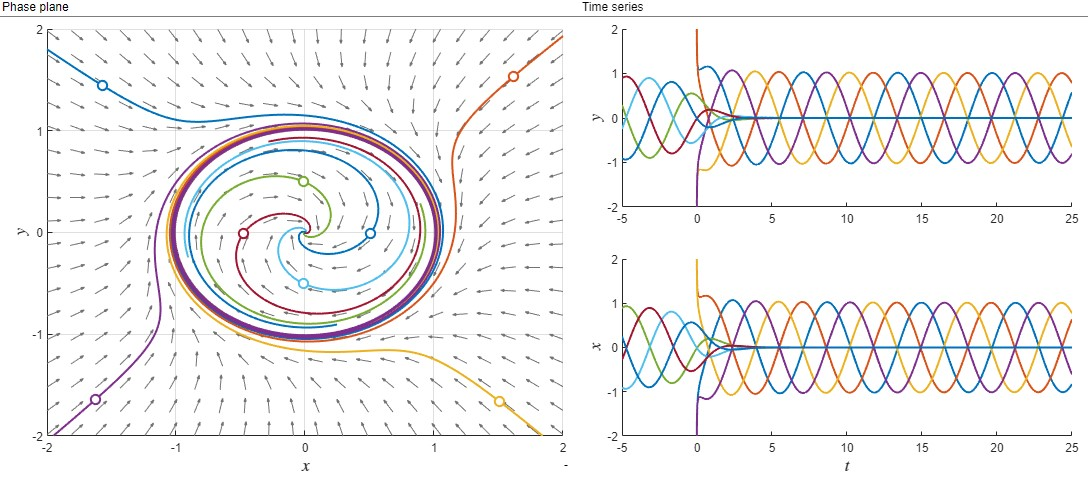
\includegraphics[width=1\textwidth]{clpe.jpg}
		\caption{Ciclo-Límite Parcialmente Estable con sentido horario de giro}
		\label{fig:clpe}
	\end{figure}\smallskip
	\newpage
	
	El Ciclo-Límite que más nos interesa es el Estable, ya que sin importar donde eligamos las condiciones iniciales siempre tenderemos a la oscilación periódica, además, si nuestro sistema sufre alguna perturbación que lo saque de la oscilación periódica siempre tenderá a reconducirse nuevamente hacia ella.
	
	\vspace{0.5cm}El estudio de los Ciclos-Límites debe hacerse de manera particular para cada sistema, primero hay que estudiar el punto de equilibrio y su estabilidad, hacer el análisis para saber si existe oscilación periódica y finalmente comprobar que dicha oscilación periódica esté aislada. No hará falta que hagamos este estudio para nuestro sistema gracias a que hemos sido capaces de escribir nuestras ecuaciones \eref{eq:sistema1} en la forma \eref{eq:sis2ec} y estas en forma canónica de Liènard \eref{eq:lienardrl}, y tenemos trabajos donde ya se hace este análisis para sistemas de este tipo (\textit{\textcolor{red}{seminal nuestro, libro amarillo, libro teruel, ponce ros 2015}}), cumpliendo una serie de condiciones en las trazas y determinantes del sistema podemos conseguir que se produzca el cambio de estabilidiad Foco Asintóticamente Estable-Centro-Foco Asintóticamente Inestable en el punto de equilibrio del sistema y por ello obteniendo el Ciclo-Límite (ya que se produce la bifurcación Foco-Centro-Ciclo Límite) (\textit{\textcolor{red}{podemos asber de antemano la estabilidad del ciclo limite? es estable, pero hay forma de saberlo antes de la experimentacion?}}) que será nuestra oscilación periódica.
		
	\newpage
	esto es texto de la siguiente hoja
	
	\chapter{Oscilación Peródica en el circuito}
	Contenido del capítulo 6.
	\newpage
	esto es texto de la siguiente hoja
	
	\chapter{TÍTULO CAPÍTULO 7}
	Contenido del capítulo 7.
	\newpage
	esto es texto de la siguiente hoja
	
	\chapter{TÍTULO CAPÍTULO 8}
	Contenido del capítulo 8.
	\newpage
	esto es texto de la siguiente hoja
	
	\chapter*{Conclusiones}
	Contenido del capítulo de conclusiones.
	\newpage
	
	
	\begin{thebibliography}{99}
		\bibitem{chuamissing1971} CHUA, L. O. Memristor – The missing circuit element. IEEE
		Transactions on Circuit Theory, 1971, vol. CT-18, no. 5, p. 507 to
		519. DOI: 10.1109/TCT.1971.1083337.
		
		\bibitem{chuaoscillator2008} Itoh, Makoto \& Chua, Leon. (2008). Memristor oscillators. I. J. Bifurcation and Chaos. 18. 3183-3206. 10.1142/S0218127408022354. 
		
		\bibitem{HP} Strukov DB, Snider GS, Stewart DR, Williams RS. The missing memristor found. Nature. 2008 May 1;453(7191):80-3. doi: 10.1038/nature06932. Erratum in: Nature. 2009 Jun 25;459(7250):1154. PMID: 18451858.
		
		\bibitem{williams} R. S. Williams, "How We Found The Missing Memristor," in IEEE Spectrum, vol. 45, no. 12, pp. 28-35, Dec. 2008, doi: 10.1109/MSPEC.2008.4687366.
		
		\bibitem{2021} Xiaoyue, Ji \& Dong, Zhekang \& Zhou, Guangdong \& Lai, Chun Sing \& Yan, Yunfeng \& Qi, Donglian. (2021). Memristive System Based Image Processing Technology: A Review and Perspective. Electronics. 10. 3176. 10.3390/electronics10243176. 
		
		\bibitem{outsiders} Caravelli, F. \& Carbajal, Juan. (2018). Memristors for the Curious Outsiders. 10.31224/osf.io/c4qr9. 
		
		\bibitem{teruel} Llibre, Jaume \& Teruel, Antonio. (2014). Introduction to the Qualitative Theory of Differential Systems: Planar, Symmetric and Continuous Piecewise Linear Systems. 10.1007/978-3-0348-0657-2. 
		
		\bibitem{docvic} Carmona, V.Bifurcaciones en Sistemas Dinámicos Lineales a Trozos. Tesis Doctoral. Universisdad de Sevilla, 2002.
		
		\bibitem{onsimplyfing} V. Carmona, E. Freire, E. Ponce and F. Torres, "On simplifying and classifying piecewise-linear systems," in IEEE Transactions on Circuits and Systems I: Fundamental Theory and Applications, vol. 49, no. 5, pp. 609-620, May 2002, doi: 10.1109/TCSI.2002.1001950.
		
		\bibitem{ponce} Amador, A., Freire, E., Ponce, E., and Ros, J., “On Discontinuous Piecewise Linear Models for Memristor Oscillators”, <i>International Journal of Bifurcation and Chaos</i>, vol. 27, no. 6, 2017. doi:10.1142/S0218127417300221.
		
	\end{thebibliography}
	
	\newpage
	
	\begin{comment}
	\chapter{Introducción}
	\begin{equation}
		\label{EcuLambda}
		y^2=3
	\end{equation}
	hola mundo prueba script prueba branch de funcion $f$ \eqref{EcuLambda} en $[2\pi]$
	\newpage
	holaaa
	\newpage
	asldkakdlkad prueba python para commit cambio
	\newpage
	\section{introa}
	holaaa
	\newpage
	\subsection{introb}
	segundo cambio tercera prueba python siguiente prueba para ver fuente
	\end{comment}
\end{document}
